% Dense validation companion manuscript scaffold.
%
% Compile from this directory:
%   latexmk -pdf dense_validation_report.tex
%
% This document is intended as a sister manuscript/report to
% DownscalingMoistureModel/paper/paper.pdf.  It deliberately treats model 6 and
% model 8 as already-defined models and focuses on dense, paddock-scale
% validation evidence.

\documentclass[11pt,a4paper]{article}

\usepackage[margin=2.5cm]{geometry}
\usepackage{graphicx}
\usepackage{booktabs}
\usepackage{amsmath}
\usepackage{microtype}
\usepackage{xcolor}
\usepackage{array}
\usepackage{tabularx}
\usepackage[round]{natbib}
\usepackage[hidelinks]{hyperref}
\usepackage{placeins}

\graphicspath{
  {../../analyses/unified_dense_validation/figures/}
  {../../analyses/unified_dense_validation/figures/stage1/}
  {../../analyses/unified_dense_validation/figures/stage1/dem_point_overlays/}
  {../../analyses/unified_dense_validation/figures/stage1/quality_surfaces/}
  {../../analyses/unified_dense_validation/figures/stage1/llara_native_prediction_maps/}
  {../../analyses/unified_dense_validation/figures/stage2_local_spiking/}
  {../../analyses/unified_dense_validation/figures/model_space_pca/}
}

\newcommand{\nse}{\ensuremath{\mathrm{NSE}}}
\newcommand{\ubrmse}{\ensuremath{\mathrm{ubRMSE}}}
\newcommand{\pearsonr}{\ensuremath{r}}
\newcommand{\vwc}{\ensuremath{\mathrm{VWC}}}
\newcommand{\modelSix}{model~6 RF}
\newcommand{\modelEight}{model~8 process}
\newcommand{\smips}{\texttt{SMIPS TotalBucket}}
\definecolor{cautioncolor}{RGB}{185,95,0}
\newcommand{\todo}[1]{\textcolor{red}{[TODO: #1]}}
\newcommand{\caution}[1]{\textcolor{cautioncolor}{[Caution: #1]}}
\newcommand{\placeholderbox}[2]{%
  \begin{center}
  \fbox{\begin{minipage}{0.92\linewidth}
  \vspace{0.7em}
  \textbf{#1}\par
  \vspace{0.35em}
  #2
  \vspace{0.7em}
  \end{minipage}}
  \end{center}
}

\title{Dense paddock-scale validation of statistical and process-based
soil-moisture downscaling}
\author{Dmitry [surname]\thanks{[affiliation; email]} \and
Yasar Adeel Ansari\thanks{[affiliation; email]}}
\date{Draft --- 1 September 2026}

\begin{document}

\maketitle

\begin{center}
\begin{minipage}{0.9\textwidth}\small\itshape
Companion validation report to ``Downscaling SMIPS soil moisture to 30\,m:
statistical and process-based estimation of root-zone soil moisture, with
validation in the Murrumbidgee catchment''.  This draft scaffold separates the
model-development evidence from the dense-site validation evidence.  Red
\todo{items} should be resolved before circulation.
\end{minipage}
\end{center}

\begin{abstract}
\todo{Write after results are stabilised. Suggested structure: one sentence on
the paddock-scale validation gap; one sentence describing Esdale, Tarrawarra,
Nerrigundah, Llara and MRI; one sentence on the model-agnostic validation table; one sentence with
headline model6/model8 skill and seasonal/wetness bias; one sentence on local
calibration/spiking; one sentence on implications for deployment.}

Root-zone soil-moisture products are increasingly evaluated against sparse
station networks, but management decisions occur at sub-property scale where
within-paddock redistribution by terrain, soil and antecedent wetness is
critical.  Here we use five retained model-ready validation datasets to test
whether the final statistical and process-based models developed in the
companion paper preserve paddock-scale soil-moisture patterns when treated as
black-box gridded predictors.  The datasets span modern dense campaign points,
historical high-density TDR grids and continuous probe networks.  Skill is
summarised using Pearson correlation ($\pearsonr$),
Nash--Sutcliffe efficiency (\nse{}), RMSE, \ubrmse{} and bias so that temporal
association, error magnitude and mean-level offsets can be separated.
\todo{Insert headline values and conclusion.}

\medskip
\noindent\textbf{Keywords:} soil moisture; dense validation; downscaling;
paddock scale; model evaluation; local calibration; Nash--Sutcliffe efficiency
\end{abstract}

\section{Introduction}\label{sec:intro}

Operational soil-moisture products generally resolve kilometres rather than
management units, yet irrigation, grazing, crop establishment
and ecophysiological modelling often require information at the scale of a
paddock or sub-property unit.  The companion paper develops two routes to
30\,m root-zone soil moisture: a statistical downscaler of the
${\approx}1$\,km \smips{} product using terrain, soil and meteorological
features, and a process-based bucket model with a static soil--terrain--climate
readout.  Its central validation question is whether these models transfer
across stations, years and spatial blocks in the OzNet monitoring network
\citep{smith2012oznet}.

That station-network validation is necessary but not sufficient for the
intended product.  Sparse stations can test regional transfer and temporal
dynamics, but they cannot directly test whether a 30\,m map reproduces
within-site moisture redistribution.  Dense point datasets provide a
``microscope'' over the downscaling field: they can reveal whether residuals
cluster by terrain position, wetness state or season, and whether competing
models fail in the same spatial locations.

This report therefore asks three questions:

\begin{enumerate}
\item \textbf{Independent paddock-scale transfer.}  When evaluated at dense
  point observations not used for model development, how much skill do
  \modelSix{} and \modelEight{} retain?
\item \textbf{Seasonal, wetness-state and terrain-conditioned bias.}  Are poor
  predictions concentrated in particular seasons, dry/wet states or
  model-input terrain/soil strata?
\item \textbf{Deployability through sparse local calibration.}  If a landholder
  can provide one or a few local sensors, how much can a separate calibration
  layer improve local prediction while preserving independent validation?
\end{enumerate}

This framing is close in spirit to two lines of previous work but differs in
its validation emphasis.  Process-oriented downscaling studies such as the
Equilibrium Moisture from Topography, Vegetation and Soil model
\citep[EMT+VS;][]{ranney2015emtvs} explicitly use fine-resolution topographic,
vegetation and soil information to redistribute coarse soil moisture to
10--100\,m scales, and show that soil and vegetation information can improve
spatial patterns when those inputs are sufficiently detailed.  Recent
machine-learning tools such as \texttt{mlhrsm} \citep{peng2024mlhrsm} instead
emphasise application-ready high-resolution mapping, uncertainty estimation and
spatial--temporal analysis from in-situ sensors, satellite products and
land-surface covariates.  The present report sits between these traditions: it
compares a statistical and a process-based 30\,m product using the same
model-agnostic dense validation table, and treats seasonal bias, wet/dry
compression and terrain-stratified error as primary validation targets rather
than secondary diagnostics.

\section{Relationship to the companion model paper}\label{sec:sister}

The purpose of this report is not to re-rank every model in the development
ladder.  Instead, it takes the two final comparison models from the companion
paper and evaluates them under a different validation geometry: dense
within-site observations.  Table~\ref{tab:sister} summarises the division of
evidence.

\begin{table}[htbp]
\centering
\caption{How this dense validation report complements the companion model
paper.}
\label{tab:sister}
\begin{tabularx}{\textwidth}{>{\raggedright\arraybackslash}X
                              >{\raggedright\arraybackslash}X}
\toprule
\textbf{Companion model paper} & \textbf{Dense validation report} \\
\midrule
Develops the full model ladder, models~1--8. &
Uses the final comparison models only: \modelSix{} and \modelEight{}. \\
Evaluates transfer across OzNet stations, spatial blocks and years. &
Evaluates transfer to independent dense point datasets at paddock scale. \\
Primary question: which validation design estimates national transfer? &
Primary question: does the 30\,m field preserve local spatial patterns and
bias structure? \\
Focuses on regional/station-level skill, residual decomposition and product
generation. &
Focuses on seasonal/wetness bias, terrain-conditioned error, spatial clustering
and sparse local adaptation. \\
Uses station-network evidence to justify final model choices. &
Uses dense-site evidence to diagnose deployment reliability and local
calibration needs. \\
\bottomrule
\end{tabularx}
\end{table}

\section{Dense validation datasets}\label{sec:data}

\subsection{Sites and validation roles}\label{sec:sites}

The analysis uses five retained model-ready validation datasets, each
contributing a different kind of evidence (Table~\ref{tab:site-inventory}).
Esdale provides the strongest modern within-site terrain coverage but only
autumn--winter dates.  Tarrawarra and Nerrigundah provide unusually dense
historical TDR campaign grids; because their raw points are denser than the
model grid, both are evaluated after aggregation to model grid-cell support.
They also carry the expected pre-\smips{} coarse-anchor caveat for
\modelSix{}.  Llara provides the strongest multi-year seasonal validation with
32 profile-mean probes across two paddocks.  MRI adds a sparser but longer
continuous probe network, useful for testing whether local calibration
behaviour holds when the spatial support is less dense.

\begin{table}[htbp]
\centering
\caption{Dense validation site inventory.  Values shown here reflect the
current analysis cache and should be checked against the final model-agnostic
tables before submission.}
\label{tab:site-inventory}
\scriptsize
\begin{tabularx}{\textwidth}{@{}>{\raggedright\arraybackslash}p{1.75cm}
                              >{\raggedright\arraybackslash}p{2.20cm}
                              rr
                              >{\raggedright\arraybackslash}p{2.35cm}
                              >{\raggedright\arraybackslash}p{1.8cm}
                              >{\raggedright\arraybackslash}X@{}}
\toprule
Site & Main role & Supports & Dates & Period & Seasons & Note \\
\midrule
Esdale & Spatial/terrain microscope & 79 & 9 & 2025-04-30--2025-07-17
  & Autumn, winter
  & Modern dense campaign; best for terrain residual inference but short
  seasonal coverage. \\
Tarrawarra & Extreme spatial-density stress test & 178 & 19
  & 1995-09-25--1996-11-29
  & Spring, summer, autumn, winter
  & 3610 raw points aggregated to model grid cells by date; \modelSix{} is
  affected by the historical coarse-anchor caveat. \\
Nerrigundah & Independent historical grid test & 128 & 12
  & 1997-08-27--1997-09-22
  & Winter, spring
  & Tarrawarra-like 15\,cm TDR campaign aggregated to model grid cells by date. \\
Llara & Seasonal/temporal microscope & 32 & 911
  & 2022-01-01--2024-06-30
  & Spring, summer, autumn, winter
  & Profile-mean probes across WE and WW paddocks; trimmed from January~2022 for
  probe-establishment QC. \\
MRI & Sparse continuous-probe transfer & 18 & 1799
  & 2021-07-01--2026-06-03
  & Spring, summer, autumn, winter
  & Mulloon Rehydration Initiative profile-mean probes; trimmed from July~2021
  for probe-establishment QC. \\
\bottomrule
\end{tabularx}
\end{table}

\begin{figure}[htbp]
\centering
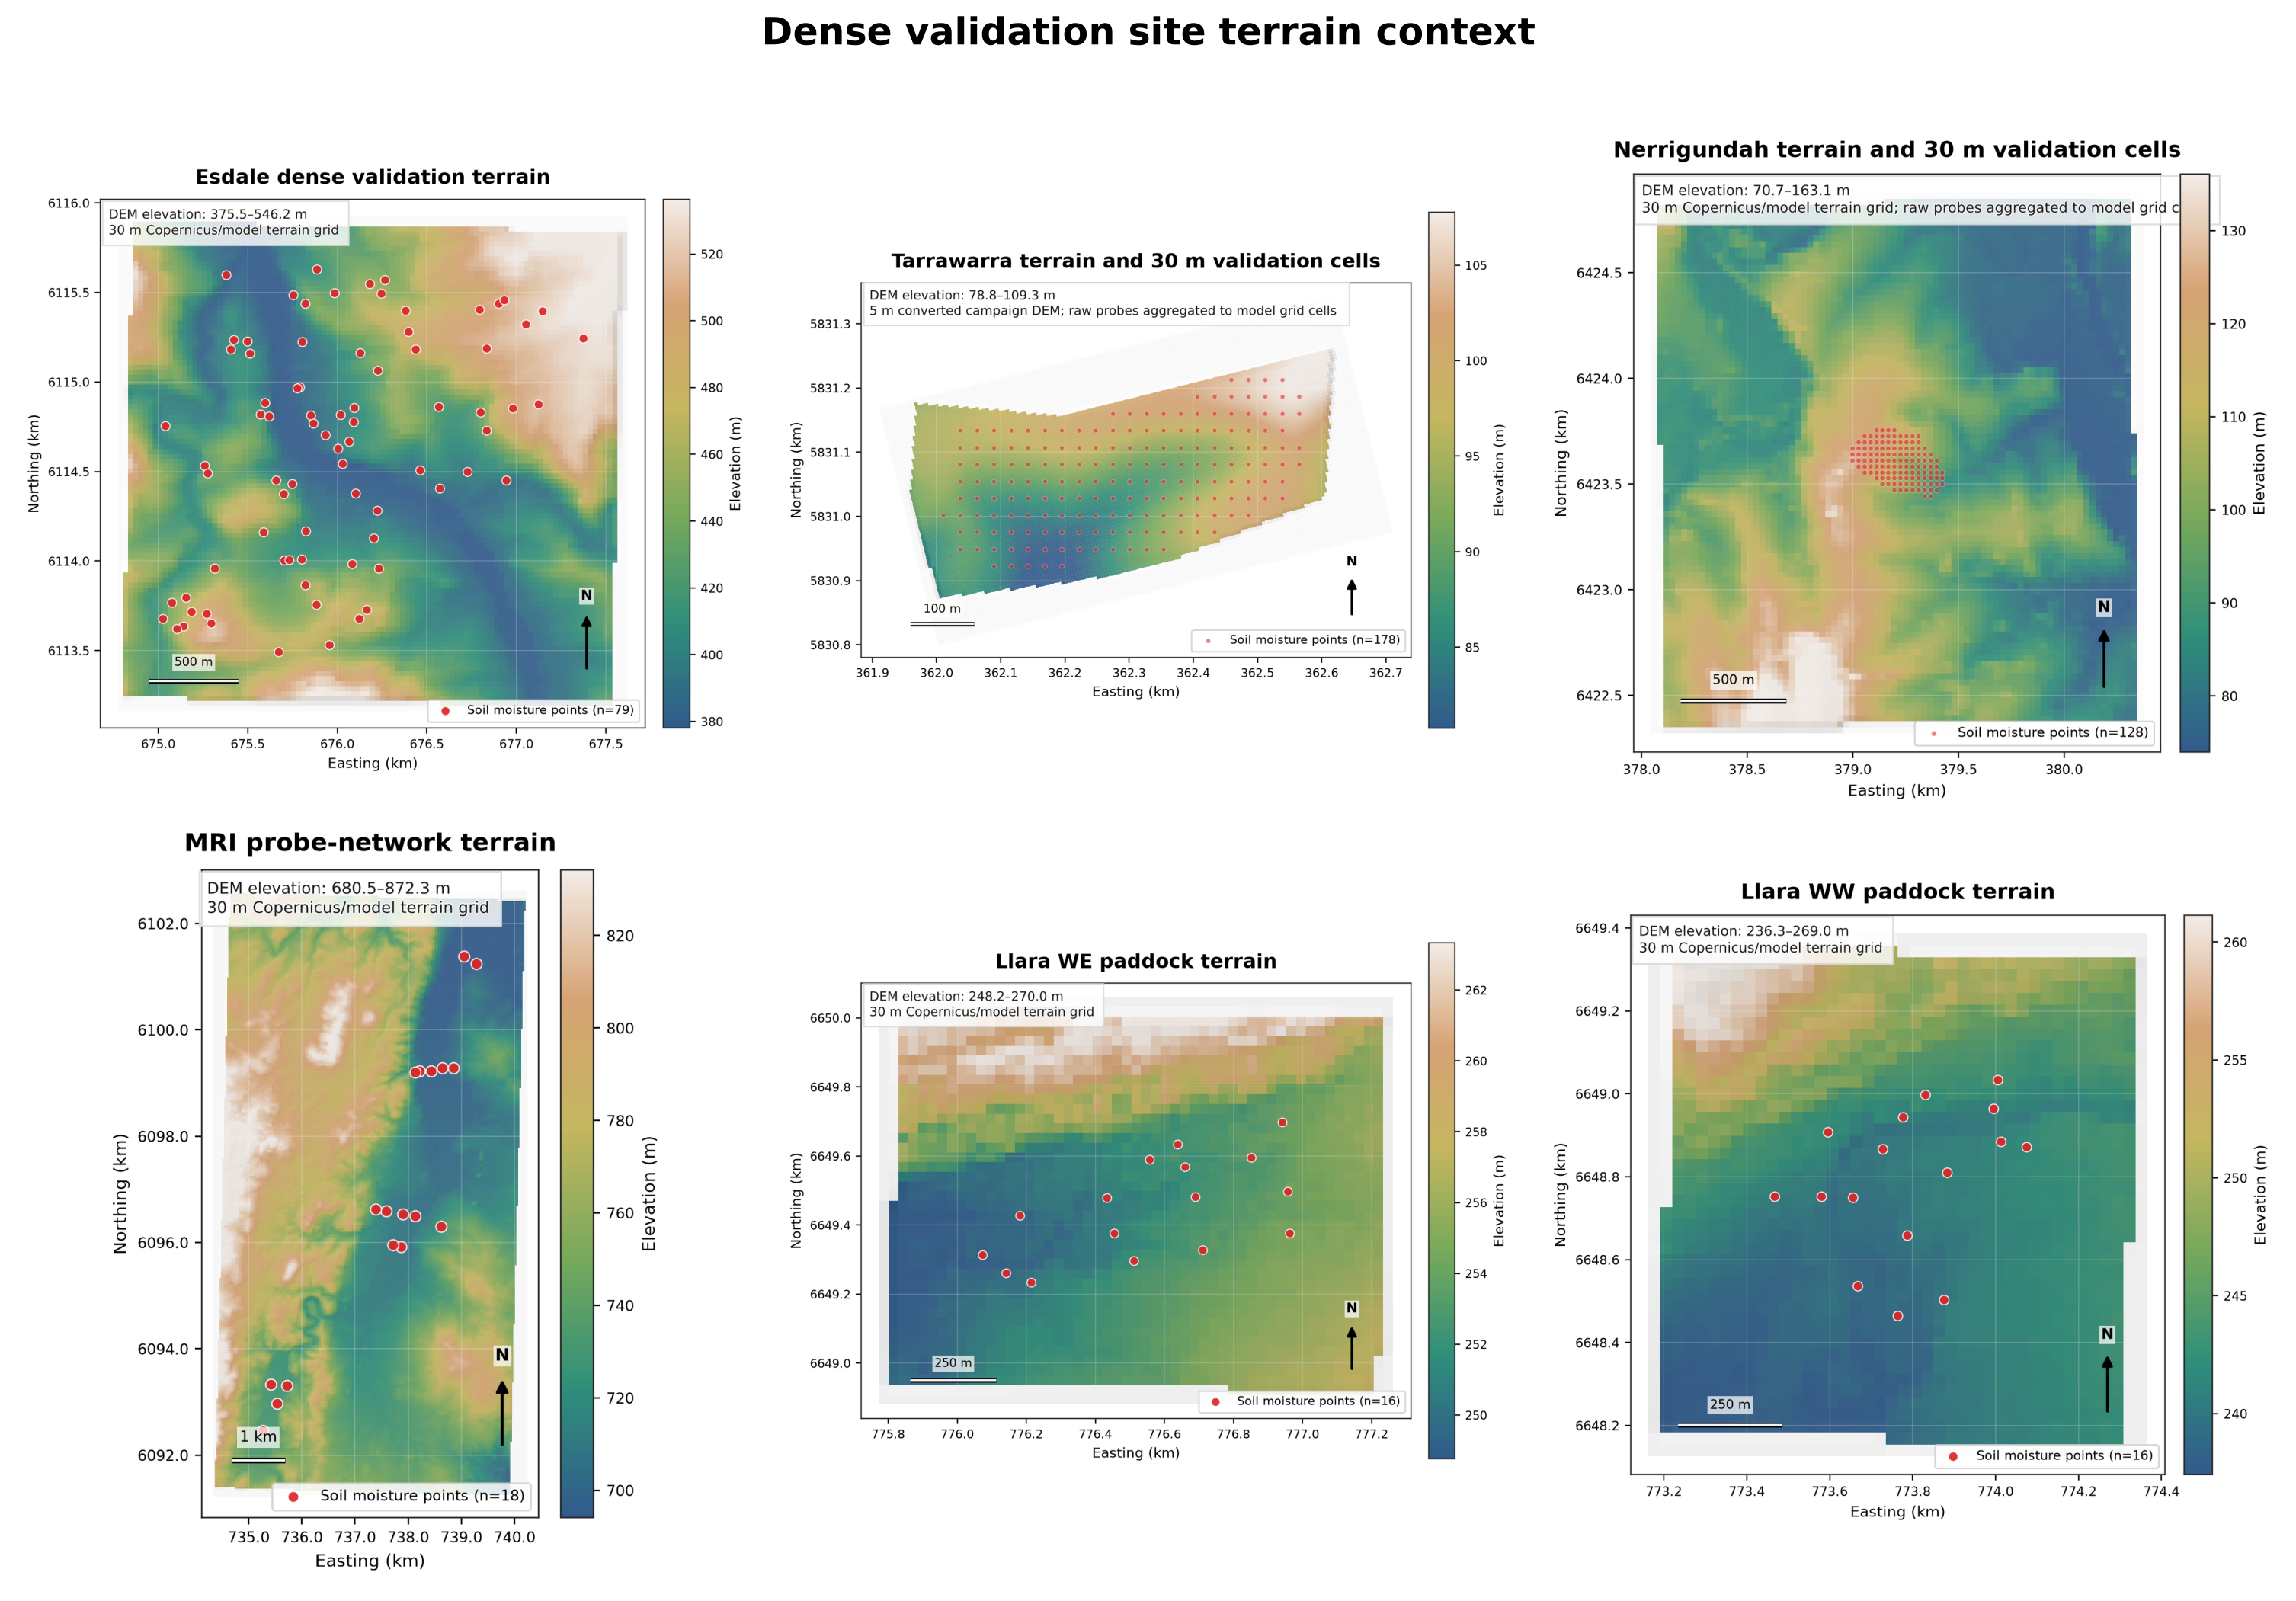
\includegraphics[width=\textwidth]{dem_points_overlay_gallery.png}
\caption{Available validation-site terrain context.  Esdale, Llara WE and
Llara WW use the 30\,m Copernicus/model terrain grid; Tarrawarra uses the
converted 5\,m campaign DEM.  Red points are soil-moisture validation supports:
probe locations for Esdale and Llara, and aggregated model-grid-cell centroids
for Tarrawarra.  \todo{Add Nerrigundah and MRI DEM panels once matching DEM
overlay rasters are staged.}}
\label{fig:dem-context}
\end{figure}

\subsection{Observation harmonisation}\label{sec:obs-harmonisation}

Each dense validation dataset measures soil moisture using methods and depth
supports that differ from each other and from the training datasets used for
the original model development.  The validation target is therefore treated as
volumetric soil moisture percentage at the best available site-specific support,
not as a perfectly interchangeable sensor quantity.

Llara and MRI measurements are obtained from continuously recording in-situ
probes.  The validation uses a profile-mean depth summary so that each
timestamp contributes a single local soil-moisture estimate.  Esdale
measurements are handheld TDR probe readings to approximately 10\,cm depth.
Tarrawarra and Nerrigundah measurements are TDR campaign readings to
approximately 15\,cm depth.

Tarrawarra and Nerrigundah also require explicit spatial-support
harmonisation.  Their campaign sampling is much denser than the model
prediction grid, so scoring raw probe observations would over-weight sub-pixel
variability that neither a 30\,m statistical model nor a 30\,m process model
can resolve.  Validation is therefore performed after aggregating observations
to the model support scale: within each model/date/grid-cell combination,
observed TDR soil moisture is averaged and the prediction is sampled once from
the corresponding raster cell.  Residual sub-pixel variation is treated as an
observational/support mismatch rather than direct model error.  This provides
an additional diagnostic: grid cells with high within-cell TDR variance mark
locations where no 30\,m model should be expected to score perfectly unless it
explicitly represents sub-pixel structure.

\subsection{Model predictions and gridded products}\label{sec:model-products}

For each site and observation date, model predictions are generated or sampled
from cached gridded products and extracted at the relevant observation support:
probe coordinates for Esdale, Llara and MRI, and model grid-cell supports for
Tarrawarra and Nerrigundah after aggregation.
The validation protocol is deliberately model agnostic: after prediction,
each model is represented only by a table of support/date predictions and
associated model-input strata.  This allows \modelSix{} and \modelEight{} to be
compared without relying on either model's internal representation.

\caution{For Tarrawarra and Nerrigundah, the current \modelSix{} prediction
tables have a \smips{}-zero/coarse-anchor caveat because historical SMIPS
coverage was unavailable or returned zero-valued inputs for the model runs.
Do not interpret their \modelSix{} skill as normal operational model6 results
unless this is resolved or explicitly framed as a coarse-anchor ablation.}

\section{Model-agnostic validation protocol}\label{sec:protocol}

\subsection{Common prediction table}\label{sec:table-schema}

All validation analyses begin from a common table with one row per
model--support--date combination:

\begin{table}[htbp]
\centering
\small
\caption{Model-agnostic prediction-table schema used by all validation steps.}
\label{tab:prediction-schema}
\begin{tabularx}{\textwidth}{>{\raggedright\arraybackslash}p{3.2cm}
                              >{\raggedright\arraybackslash}X}
\toprule
Field group & Required / derived columns \\
\midrule
Identity & Site, model name, support identifier (probe or grid cell) and
sampling date. \\
Location & Longitude, latitude and optional projected coordinates. \\
Target and prediction & Observed soil moisture, predicted soil moisture and
residual, defined as prediction minus observation. \\
Temporal strata & season, year, date block, wetness state \\
Static model inputs & elevation, slope, TWI, HLI, accumulation, aspect
components, SLGA soil properties \\
Dynamic model inputs & SMIPS summaries where available, antecedent rainfall,
PET and VPD summaries \\
\bottomrule
\end{tabularx}
\end{table}

\subsection{Metrics}\label{sec:metrics}

Skill is quantified with five complementary metrics:

\begin{align}
\pearsonr &= \frac{\sum_i (y_i - \bar{y})(\hat{y}_i - \bar{\hat{y}})}
  {\sqrt{\sum_i (y_i - \bar{y})^2}\sqrt{\sum_i(\hat{y}_i - \bar{\hat{y}})^2}}, \\
\nse &= 1 - \frac{\sum_i (y_i - \hat{y}_i)^2}
               {\sum_i (y_i - \bar{y})^2}, \\
\mathrm{RMSE} &= \sqrt{\frac{1}{n}\sum_i (y_i - \hat{y}_i)^2}, \\
\mathrm{bias} &= \frac{1}{n}\sum_i(\hat{y}_i - y_i), \\
\ubrmse &= \sqrt{\max(\mathrm{RMSE}^2 - \mathrm{bias}^2, 0)}.
\end{align}

Here $y_i$ is observed soil moisture and $\hat{y}_i$ is predicted soil
moisture.  We report pooled metrics by site and model, seasonal metrics,
per-support metrics and paired model differences at matched support/date rows.
Pearson $\pearsonr$ measures whether predictions track temporal or spatial
variation, whereas the Nash--Sutcliffe efficiency \citep[\nse;][]{nash1970river}
penalises both variance errors and mean-level offsets.  Where observed variance
is low, \nse{} can be unstable or harsh; interpretation therefore uses Pearson
$\pearsonr$, RMSE, \ubrmse{} and bias alongside \nse{}.

\subsection{Blocking and separation of validation from calibration}
\label{sec:blocking}

Stage~1 uses all dense observations only as external validation.  Stage~2 uses
controlled local calibration subsets but validates on held-out points and dates.
The strict spatial+temporal block is treated as the meaningful transfer
estimate because it tests whether calibration learned a transferable local
relationship rather than memorising a point or date.

\section{Stage 1: independent dense-point validation}\label{sec:stage1}

Before interpreting scalar validation metrics, it is useful to see the gridded
objects being scored.  Figures~\ref{fig:esdale-dry-wet} and
\ref{fig:tarrawarra-dry-wet} show the driest and wettest observed campaign dates
for Esdale and Tarrawarra, respectively, with the coarse estimate, \modelSix{}
and \modelEight{} shown side by side.  These panels are intended as a visual
orientation to the map products; all scores below are calculated from matched
validation supports rather than from visual inspection.

\begin{figure}[htbp]
\centering
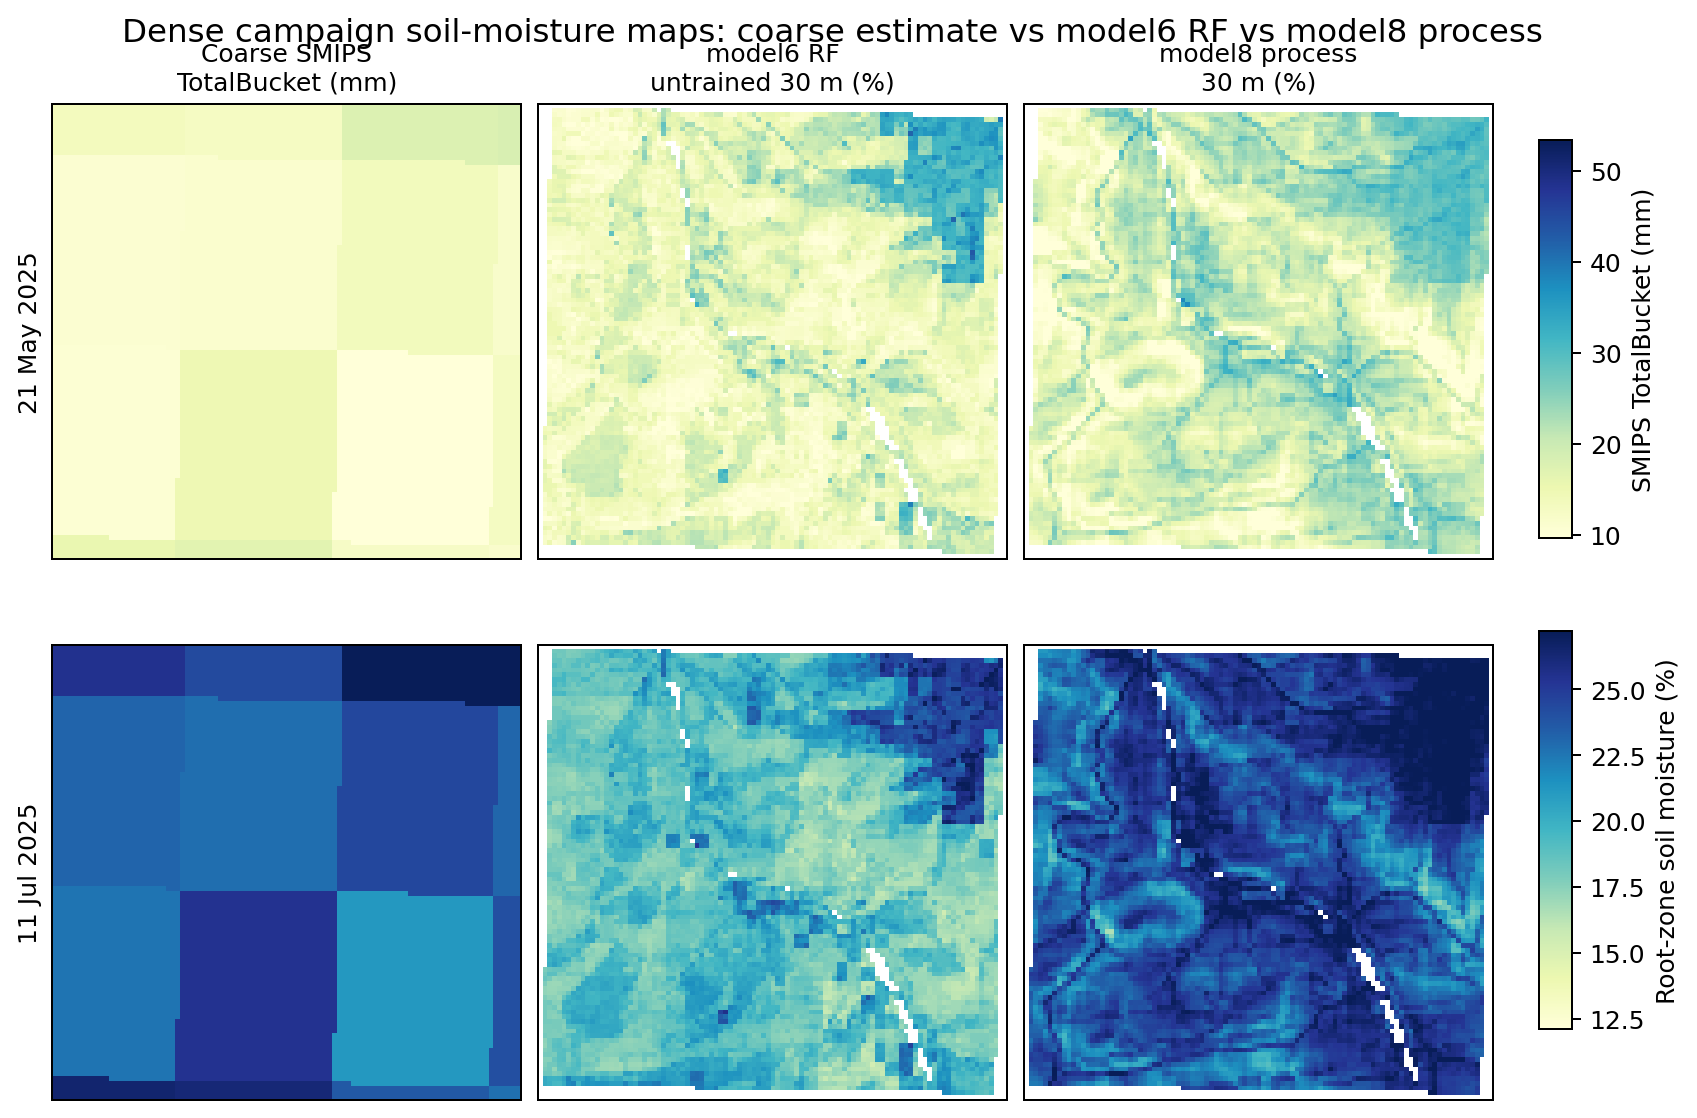
\includegraphics[width=\textwidth]{esdale_dry_wet_coarse_model6_model8_gallery.png}
\caption{Esdale gridded prediction overview for the observed driest
(21~May~2025; mean observed soil moisture 7.0\,\%) and wettest
(11~July~2025; 23.2\,\%) dense-campaign dates.  Columns show the coarse SMIPS
estimate, \modelSix{} and \modelEight{}.}
\label{fig:esdale-dry-wet}
\end{figure}

\begin{figure}[htbp]
\centering
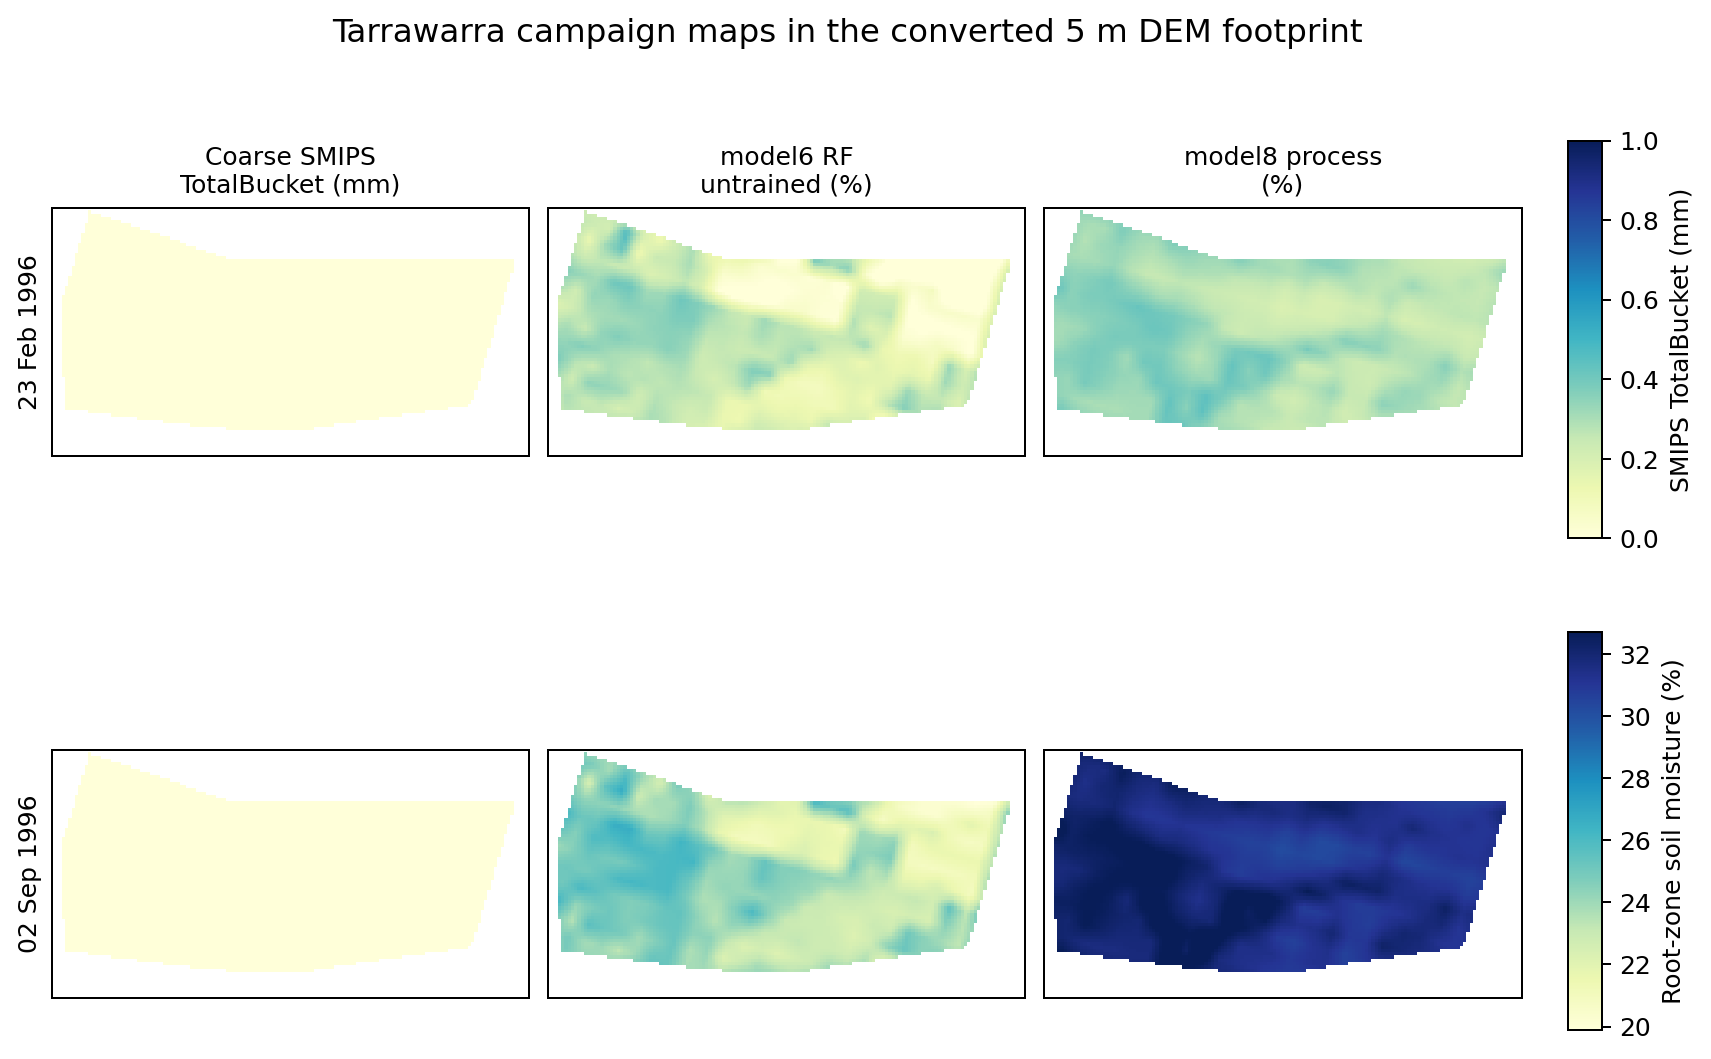
\includegraphics[width=\textwidth]{tarrawarra_dry_wet_coarse_model6_model8_gallery.png}
\caption{Tarrawarra gridded prediction overview for the observed driest
(23~February~1996; mean observed soil moisture 20.3\,\%) and wettest
(2~September~1996; 48.4\,\%) campaign dates after aggregation to model-grid
support.  Columns show the historical coarse estimate, \modelSix{} and
\modelEight{}.  \caution{The historical \smips{} input is affected by the
zero-valued coarse-anchor caveat for this run.}}
\label{fig:tarrawarra-dry-wet}
\end{figure}

\begin{figure}[htbp]
\centering
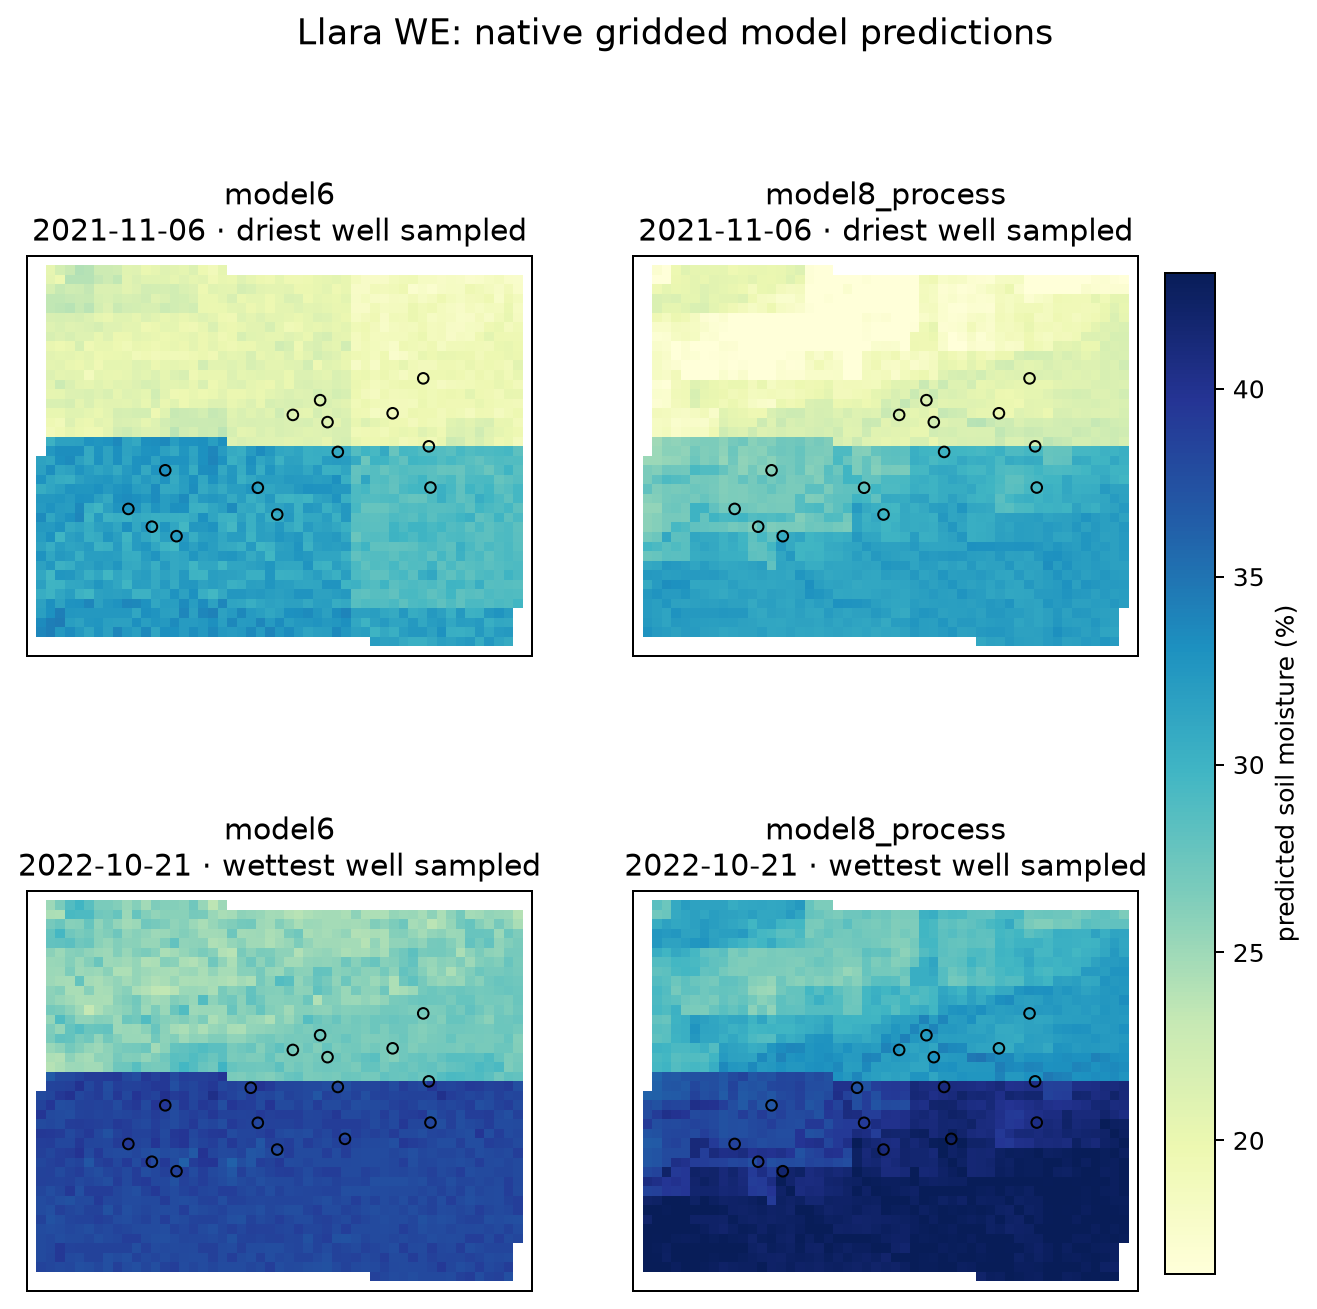
\includegraphics[width=0.49\textwidth]{llara_WE_native_prediction_gallery.png}
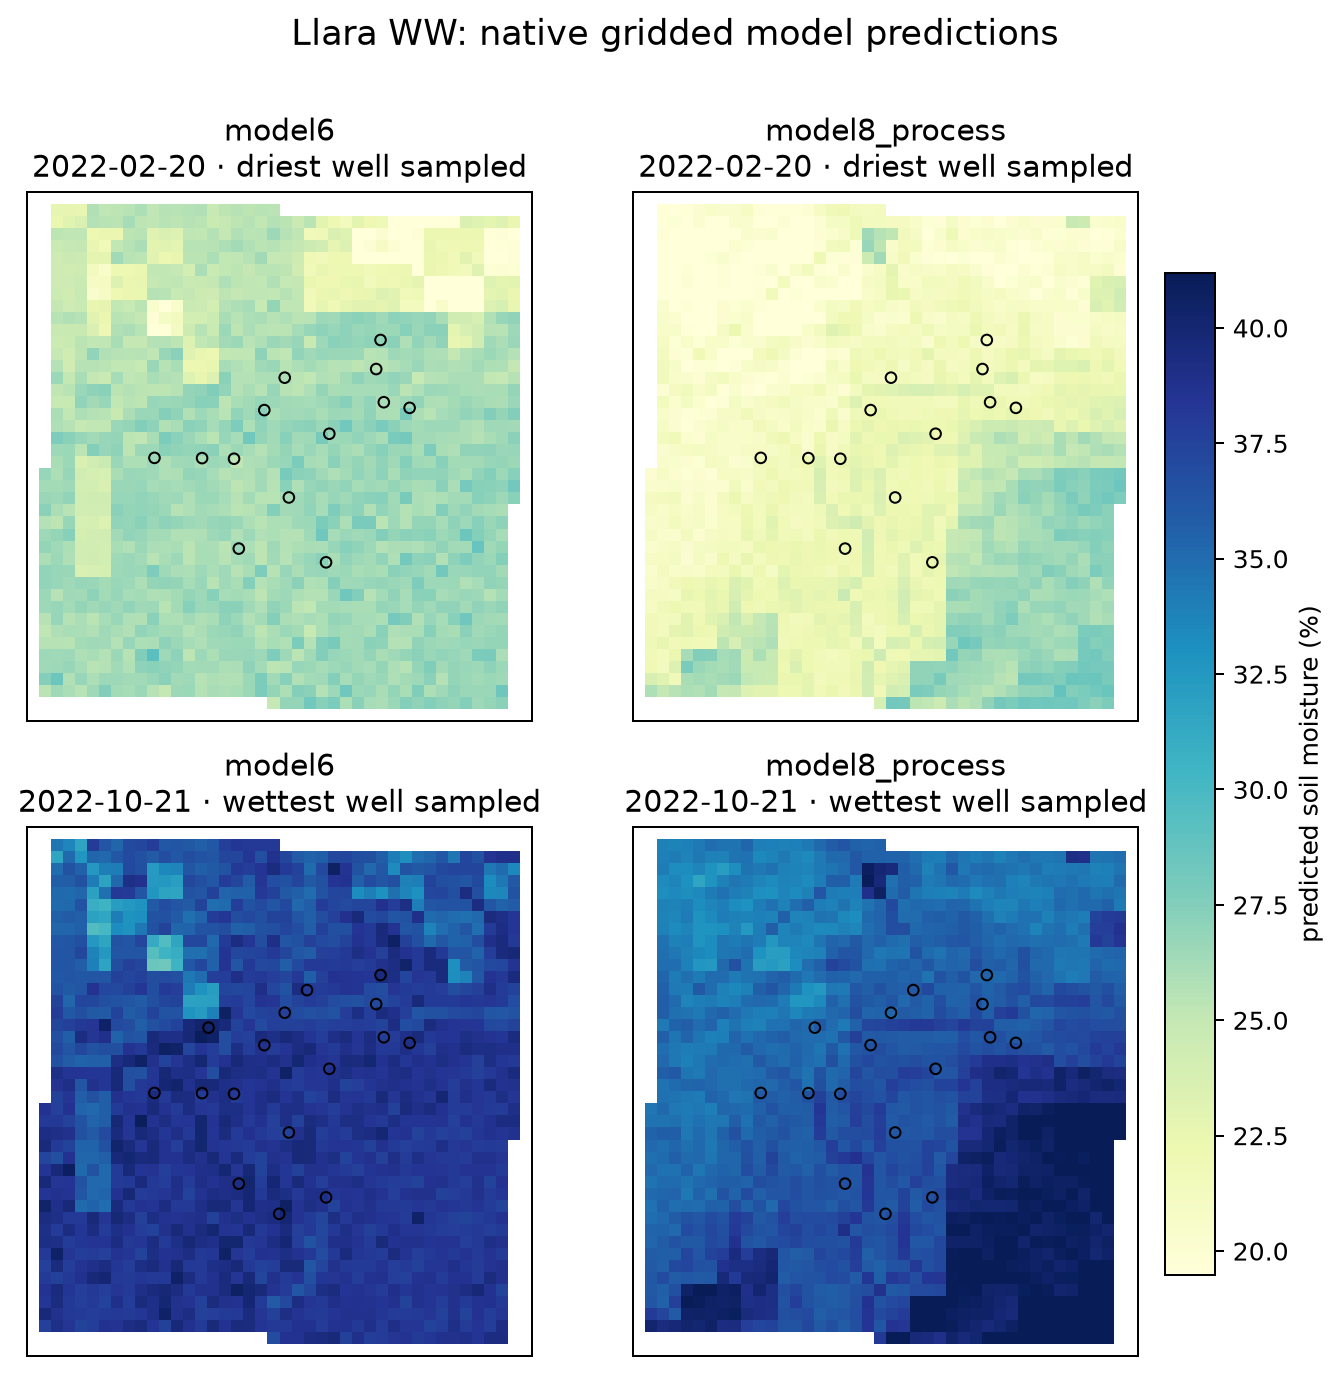
\includegraphics[width=0.49\textwidth]{llara_WW_native_prediction_gallery.png}
\caption{Llara gridded prediction examples for the WE and WW paddocks,
shown separately.  \todo{Consider separate full-width panels in final layout if
the two-paddock figure is too dense.}}
\label{fig:llara-gridded}
\end{figure}

\FloatBarrier

\subsection{Headline site-level skill}\label{sec:stage1-headline}

The first analysis pools all available support/date rows by site and model
(Fig.~\ref{fig:overall-skill}).  This figure should be interpreted as an
external paddock-scale validation summary, not as a replacement for the OzNet
cross-validation ladder in the companion paper.

\begin{figure}[htbp]
\centering
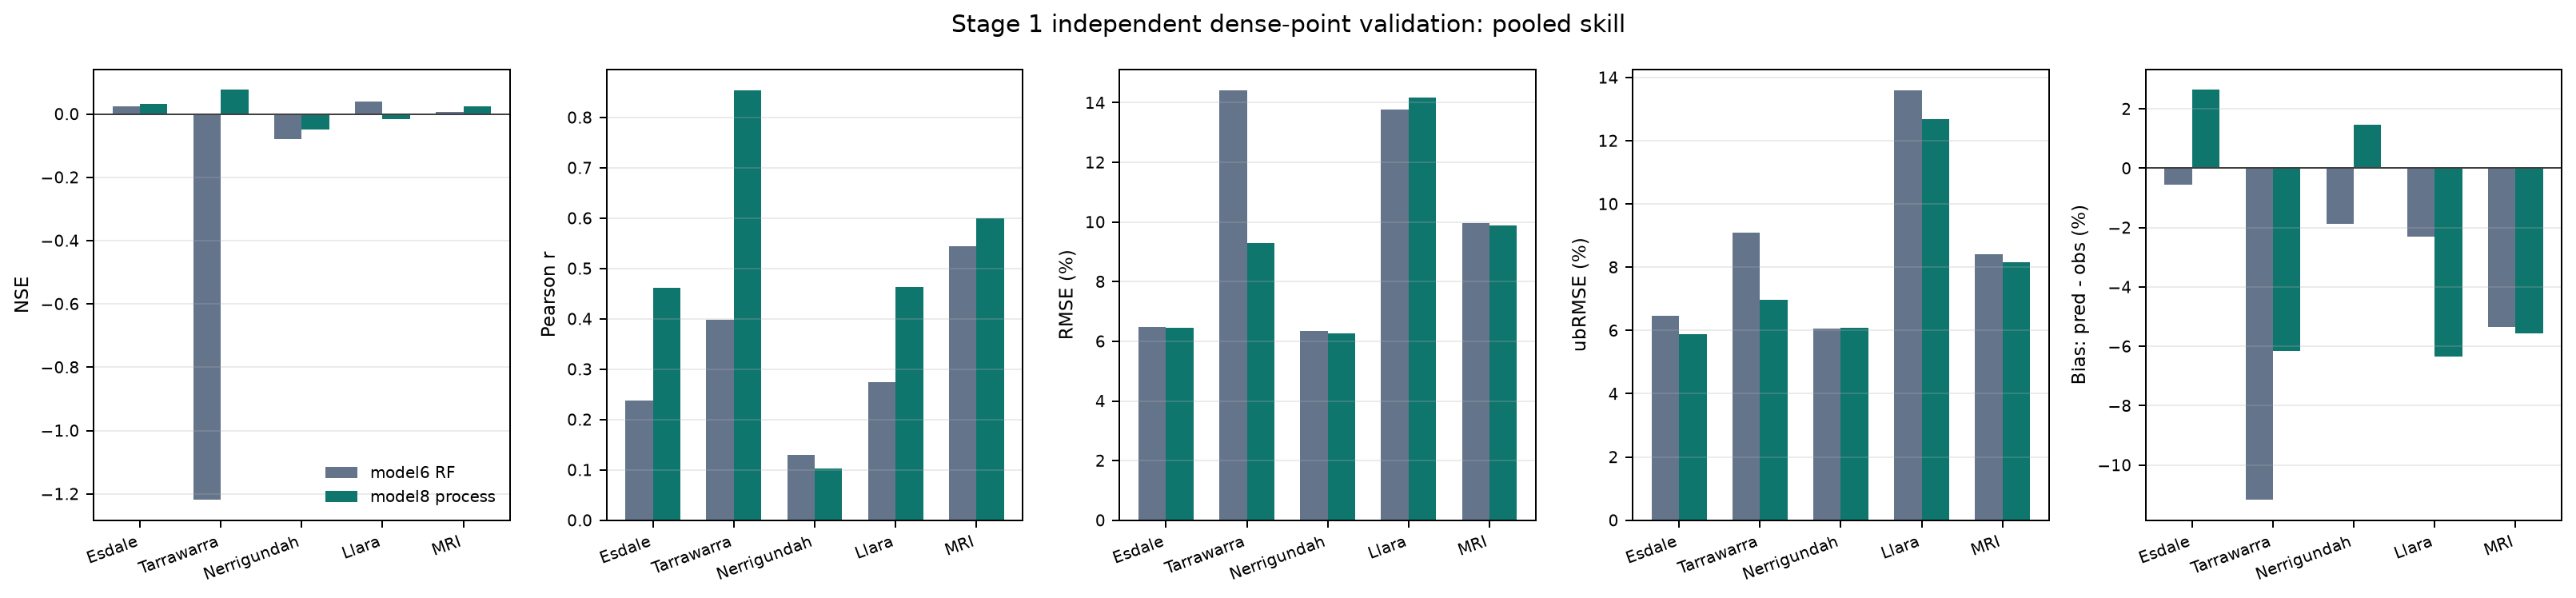
\includegraphics[width=\textwidth]{site_model_overall_skill.png}
\caption{Stage~1 independent dense-point validation: pooled \nse{}, Pearson
$\pearsonr$, RMSE, \ubrmse{} and bias by site and model.  The five metrics are
reported together because correlation, efficiency, total error magnitude,
bias-corrected error and mean-level offset answer different validation
questions.}
\label{fig:overall-skill}
\end{figure}

The headline result is that validation-site transfer remains modest at this
scale.  Across the five retained datasets, pooled \nse{} is near zero for most
site/model combinations despite positive Pearson correlations, meaning that
the models often track some spatial or temporal ordering without yet
reproducing the full observed magnitude and offset.  Esdale and Nerrigundah
have the lowest RMSE, approximately 6--6.5 volumetric percentage points, but
Nerrigundah has weak correlation for both models.  Tarrawarra shows the clearest
advantage for \modelEight{} after grid-cell support aggregation, while Llara
and MRI show stronger temporal association for \modelEight{} but only modest
differences in total RMSE.  The historical campaign sites remain especially
useful as stress tests of spatial structure, whereas Llara and MRI are the
stronger tests of continuous temporal behaviour.

\begin{table}[htbp]
\centering
\small
\caption{Headline independent validation metrics from the current unified
analysis cache.  For Tarrawarra and Nerrigundah, $n$ is the number of
model/date/grid-cell supports after aggregation, not the number of raw TDR
observations.  Llara and MRI are QC-trimmed to 2022-01-01 and 2021-07-01,
respectively.}
\label{tab:headline-metrics}
\begin{tabularx}{\textwidth}{llrrrrrX}
\toprule
Site & Model & $n$ & \nse{} & $\pearsonr$ & RMSE & \ubrmse{} & Bias / interpretation \\
\midrule
Esdale & \modelSix{} & 560 & 0.023 & 0.238 & 6.477 & 6.453
  & $-0.558$; weak spatial skill, small mean dry bias. \\
Esdale & \modelEight{} & 560 & 0.031 & 0.462 & 6.452 & 5.884
  & $2.645$; higher association but wet-biased. \\
Tarrawarra & \modelSix{} & 2154 & -1.219 & 0.398 & 14.402 & 9.093
  & $-11.169$; strong dry bias, interpreted with the \smips{}-zero caveat. \\
Tarrawarra & \modelEight{} & 2154 & 0.077 & 0.853 & 9.291 & 6.958
  & $-6.157$; strongest Tarrawarra association after support aggregation. \\
Nerrigundah & \modelSix{} & 1536 & -0.079 & 0.130 & 6.341 & 6.054
  & $-1.887$; low RMSE but weak association under the historical-grid test. \\
Nerrigundah & \modelEight{} & 1536 & -0.050 & 0.102 & 6.254 & 6.078
  & $1.476$; slightly lower RMSE but still weak association. \\
Llara & \modelSix{} & 28390 & 0.039 & 0.274 & 13.777 & 13.582
  & $-2.308$; slightly better error/bias than \modelEight{} overall. \\
Llara & \modelEight{} & 28390 & -0.017 & 0.463 & 14.172 & 12.677
  & $-6.335$; stronger association but larger dry bias. \\
MRI & \modelSix{} & 29046 & 0.006 & 0.545 & 9.972 & 8.413
  & $-5.354$; moderate temporal association with dry bias. \\
MRI & \modelEight{} & 29046 & 0.024 & 0.600 & 9.882 & 8.157
  & $-5.577$; slightly better efficiency/correlation, similar dry bias. \\
\bottomrule
\end{tabularx}
\end{table}

\subsection{Paired comparison of model6 and model8}\label{sec:stage1-paired}

Because \modelSix{} and \modelEight{} are sampled at the same support/date rows,
their residuals can be compared pairwise.  The main paired comparison reports
RMSE(\modelSix{})--RMSE(\modelEight{}) and
bias(\modelSix{})--bias(\modelEight{}) on matched supports, with bootstrap
uncertainty added in the supplement where appropriate.  Positive RMSE
differences indicate lower RMSE for \modelEight{}; positive bias differences
indicate that \modelSix{} is wetter, or less dry, than \modelEight{} on the
same matched rows.

\placeholderbox{Planned paired-comparison figure}{
Create a compact paired model figure with one row per site.  Suggested panels:
RMSE(\modelSix{})--RMSE(\modelEight{}), bias(\modelSix{})--bias(\modelEight{}),
and optionally bootstrap intervals for these paired residual summaries.  Source
table:
\nolinkurl{outputs/unified_dense_validation/stage1_independent_validation/paired_model_comparison_overall.csv}.}

\subsection{Predicted and observed time series}\label{sec:stage1-timeseries}

Spatially averaged time series provide a diagnostic of seasonal tracking and
mean-level bias.  They are not a substitute for support-level scoring, but they
make temporal drift and wet/dry compression visually apparent.

\begin{figure}[htbp]
\centering
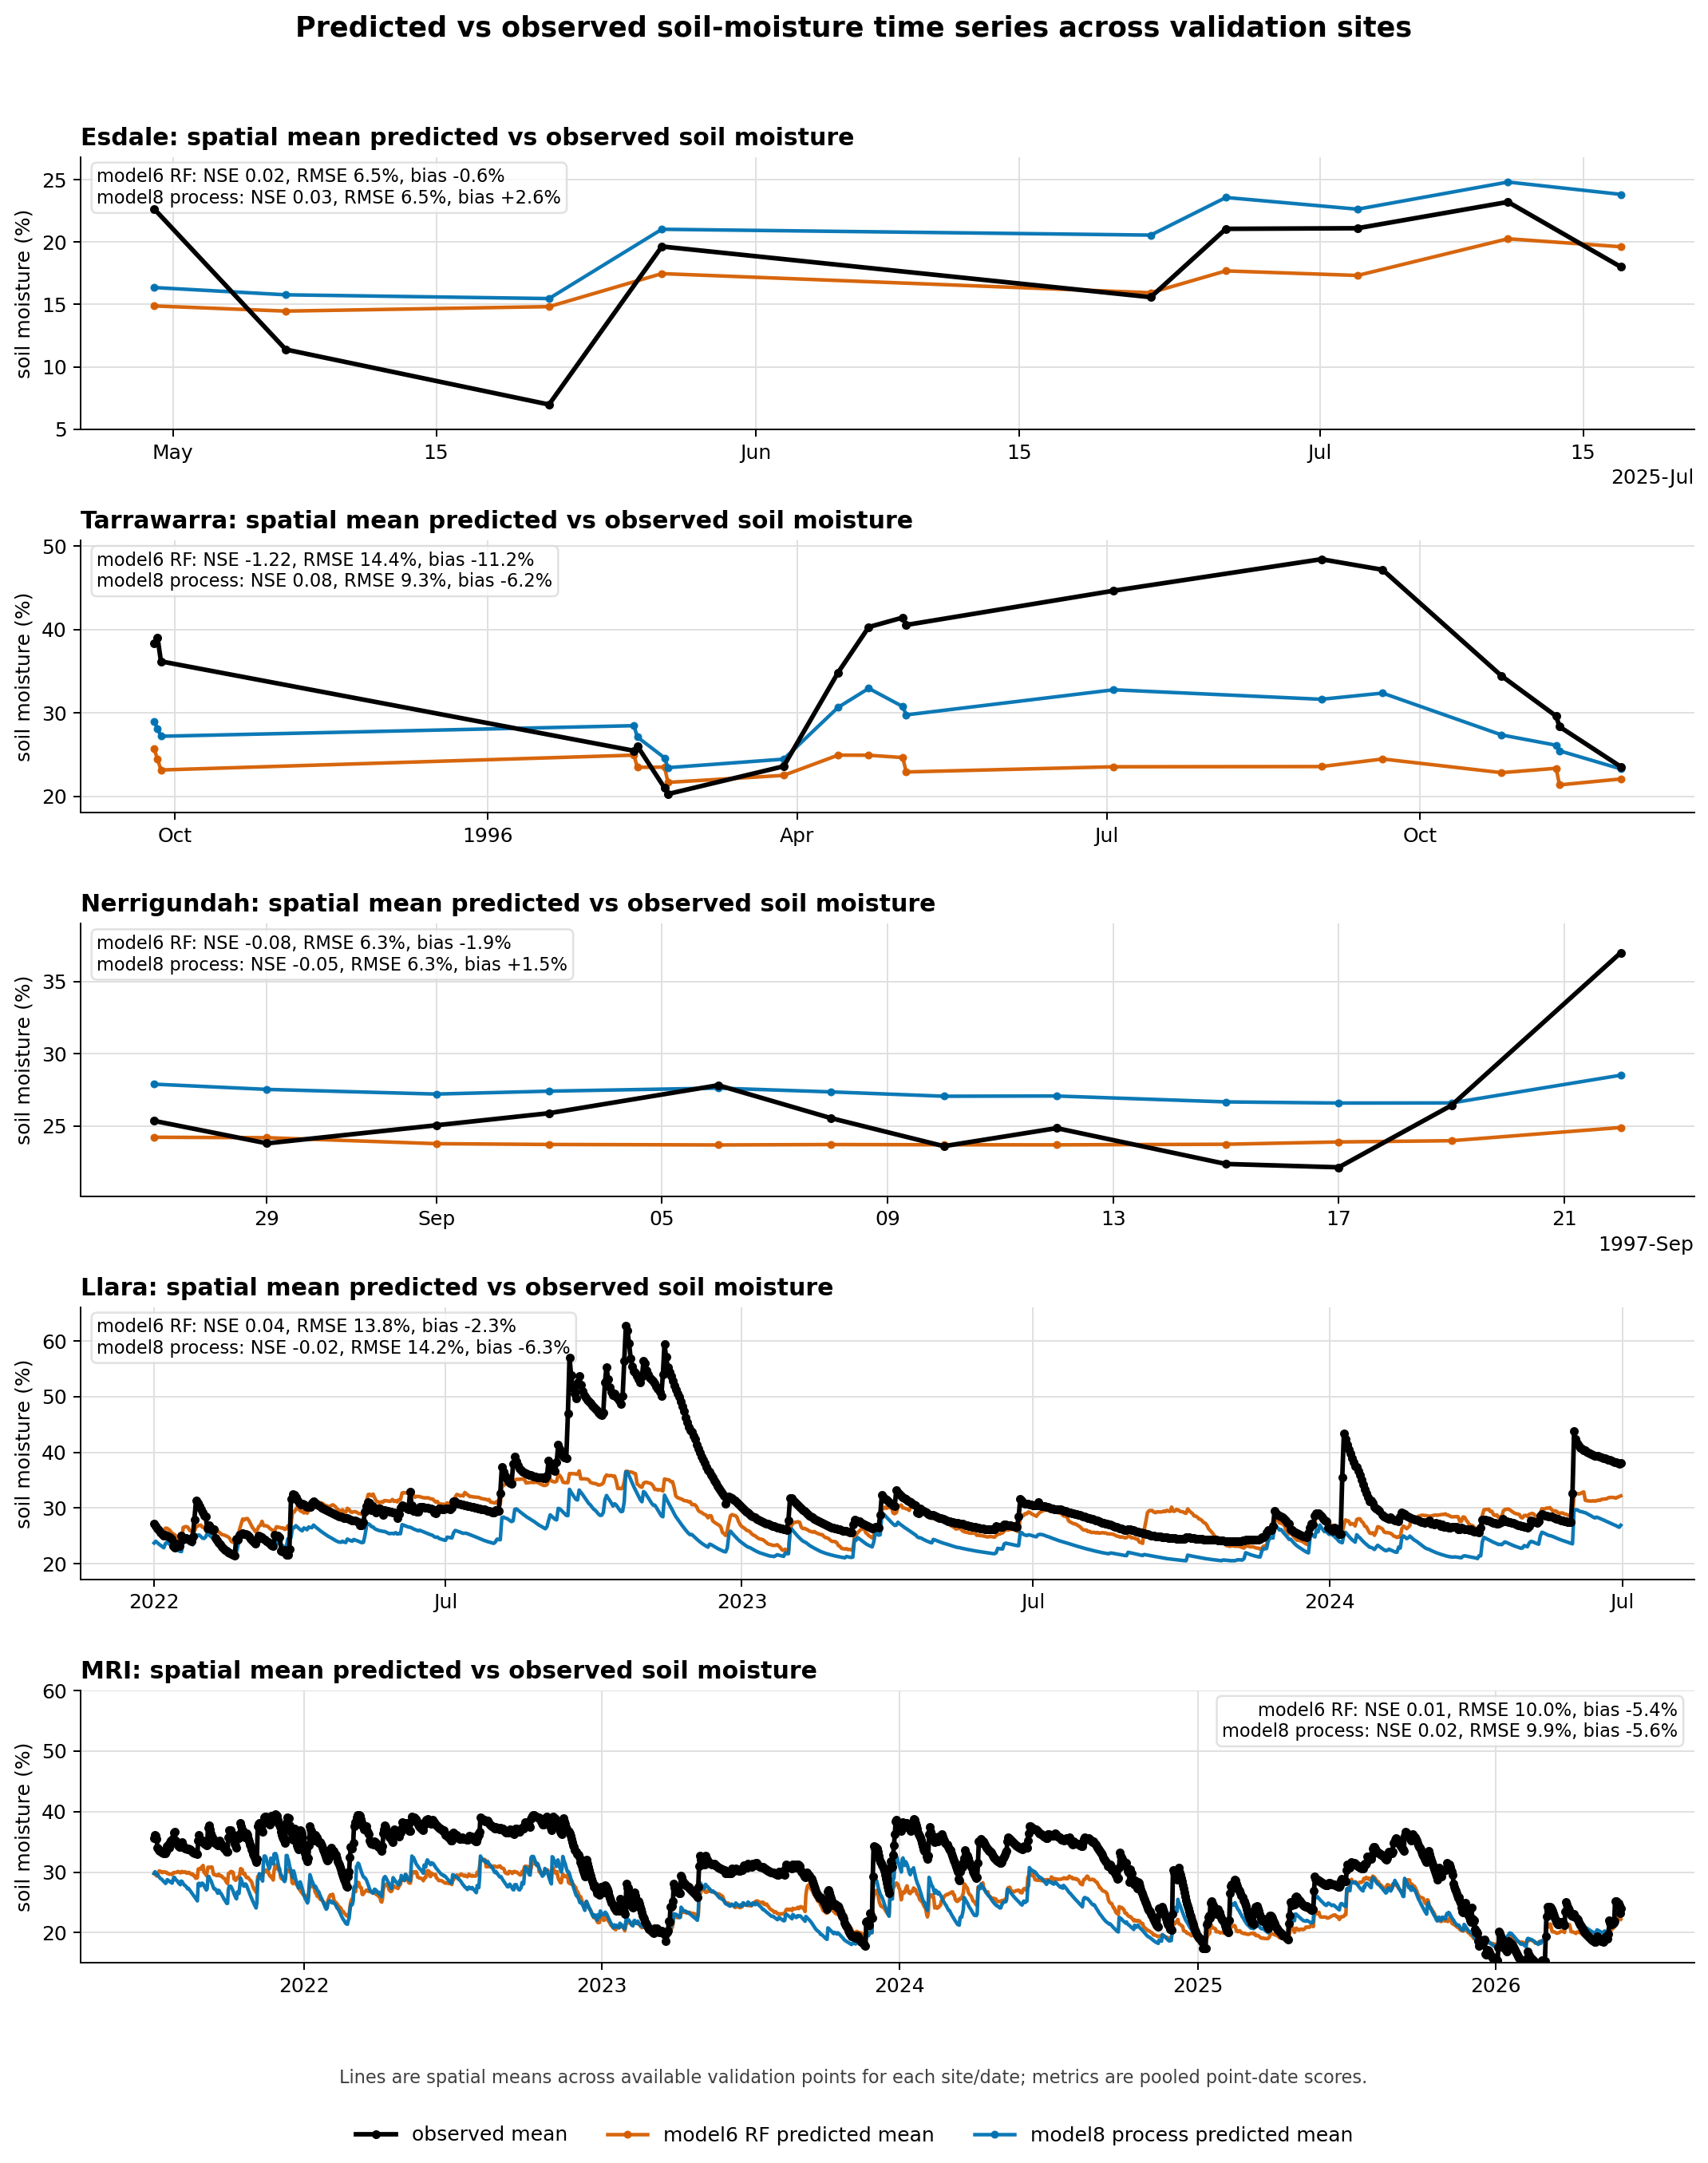
\includegraphics[width=\textwidth]{predicted_vs_observed_timeseries_validation_sites.png}
\caption{Observed and predicted soil-moisture time series by site.  Values are
spatial means over available validation points for each date.  \todo{Check
whether Llara should be shown as WE/WW paddocks separately in the final
manuscript.}}
\label{fig:timeseries}
\end{figure}

\subsection{Seasonal and wetness-state bias}\label{sec:stage1-seasonal}

The dense validation should emphasise seasonal and wetness-state bias because
a model can have acceptable pooled error while systematically overpredicting
dry states or underpredicting wet states.  This is particularly relevant to
trafficability, drought stress and paddock management decisions.

Seasonal residuals show that mean bias is not stable through time
(Fig.~\ref{fig:seasonal-bias}).  Esdale is limited to autumn--winter, where
\modelSix{} changes from a small autumn wet bias to a winter dry bias, while
\modelEight{} remains wetter than observed in both seasons.  Tarrawarra is
dominated by the \modelSix{} historical coarse-anchor caveat; \modelSix{} is
strongly dry in spring, autumn and winter but close to neutral in summer, while
\modelEight{} is still dry in spring, autumn and winter and wet-biased in
summer.  Nerrigundah provides only winter--spring campaign dates, so it is best
read as an independent historical grid check rather than a full seasonal
diagnostic.  Llara and MRI provide the strongest multi-year seasonal tests;
both show persistent dry bias in the continuous-probe records, especially for
\modelEight{}.

\begin{figure}[htbp]
\centering
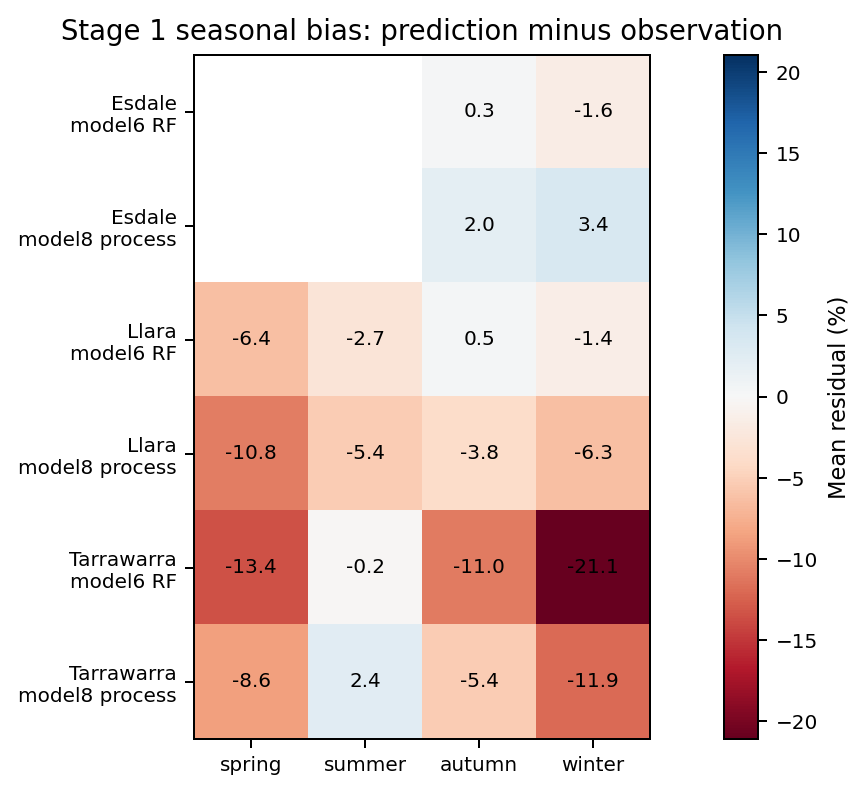
\includegraphics[width=0.92\textwidth]{seasonal_bias_by_site_model.png}
\caption{Seasonal bias by site and model.  Residuals are prediction minus
observation; positive values indicate overprediction.  \todo{In final caption,
name the largest seasonal biases and note which site has insufficient seasonal
coverage.}}
\label{fig:seasonal-bias}
\end{figure}

Wetness-state residuals indicate a general compression of the observed
moisture range (Fig.~\ref{fig:wetness-bias}).  The models tend to overpredict
the driest observed quartile and underpredict the wettest observed quartile,
with the effect particularly visible in the longer probe records and the
historical campaign grids.  This pattern is important because a map that gets
the mid-range approximately right may still misrepresent the very wet and very
dry paddock positions that often drive management decisions.

\begin{figure}[htbp]
\centering
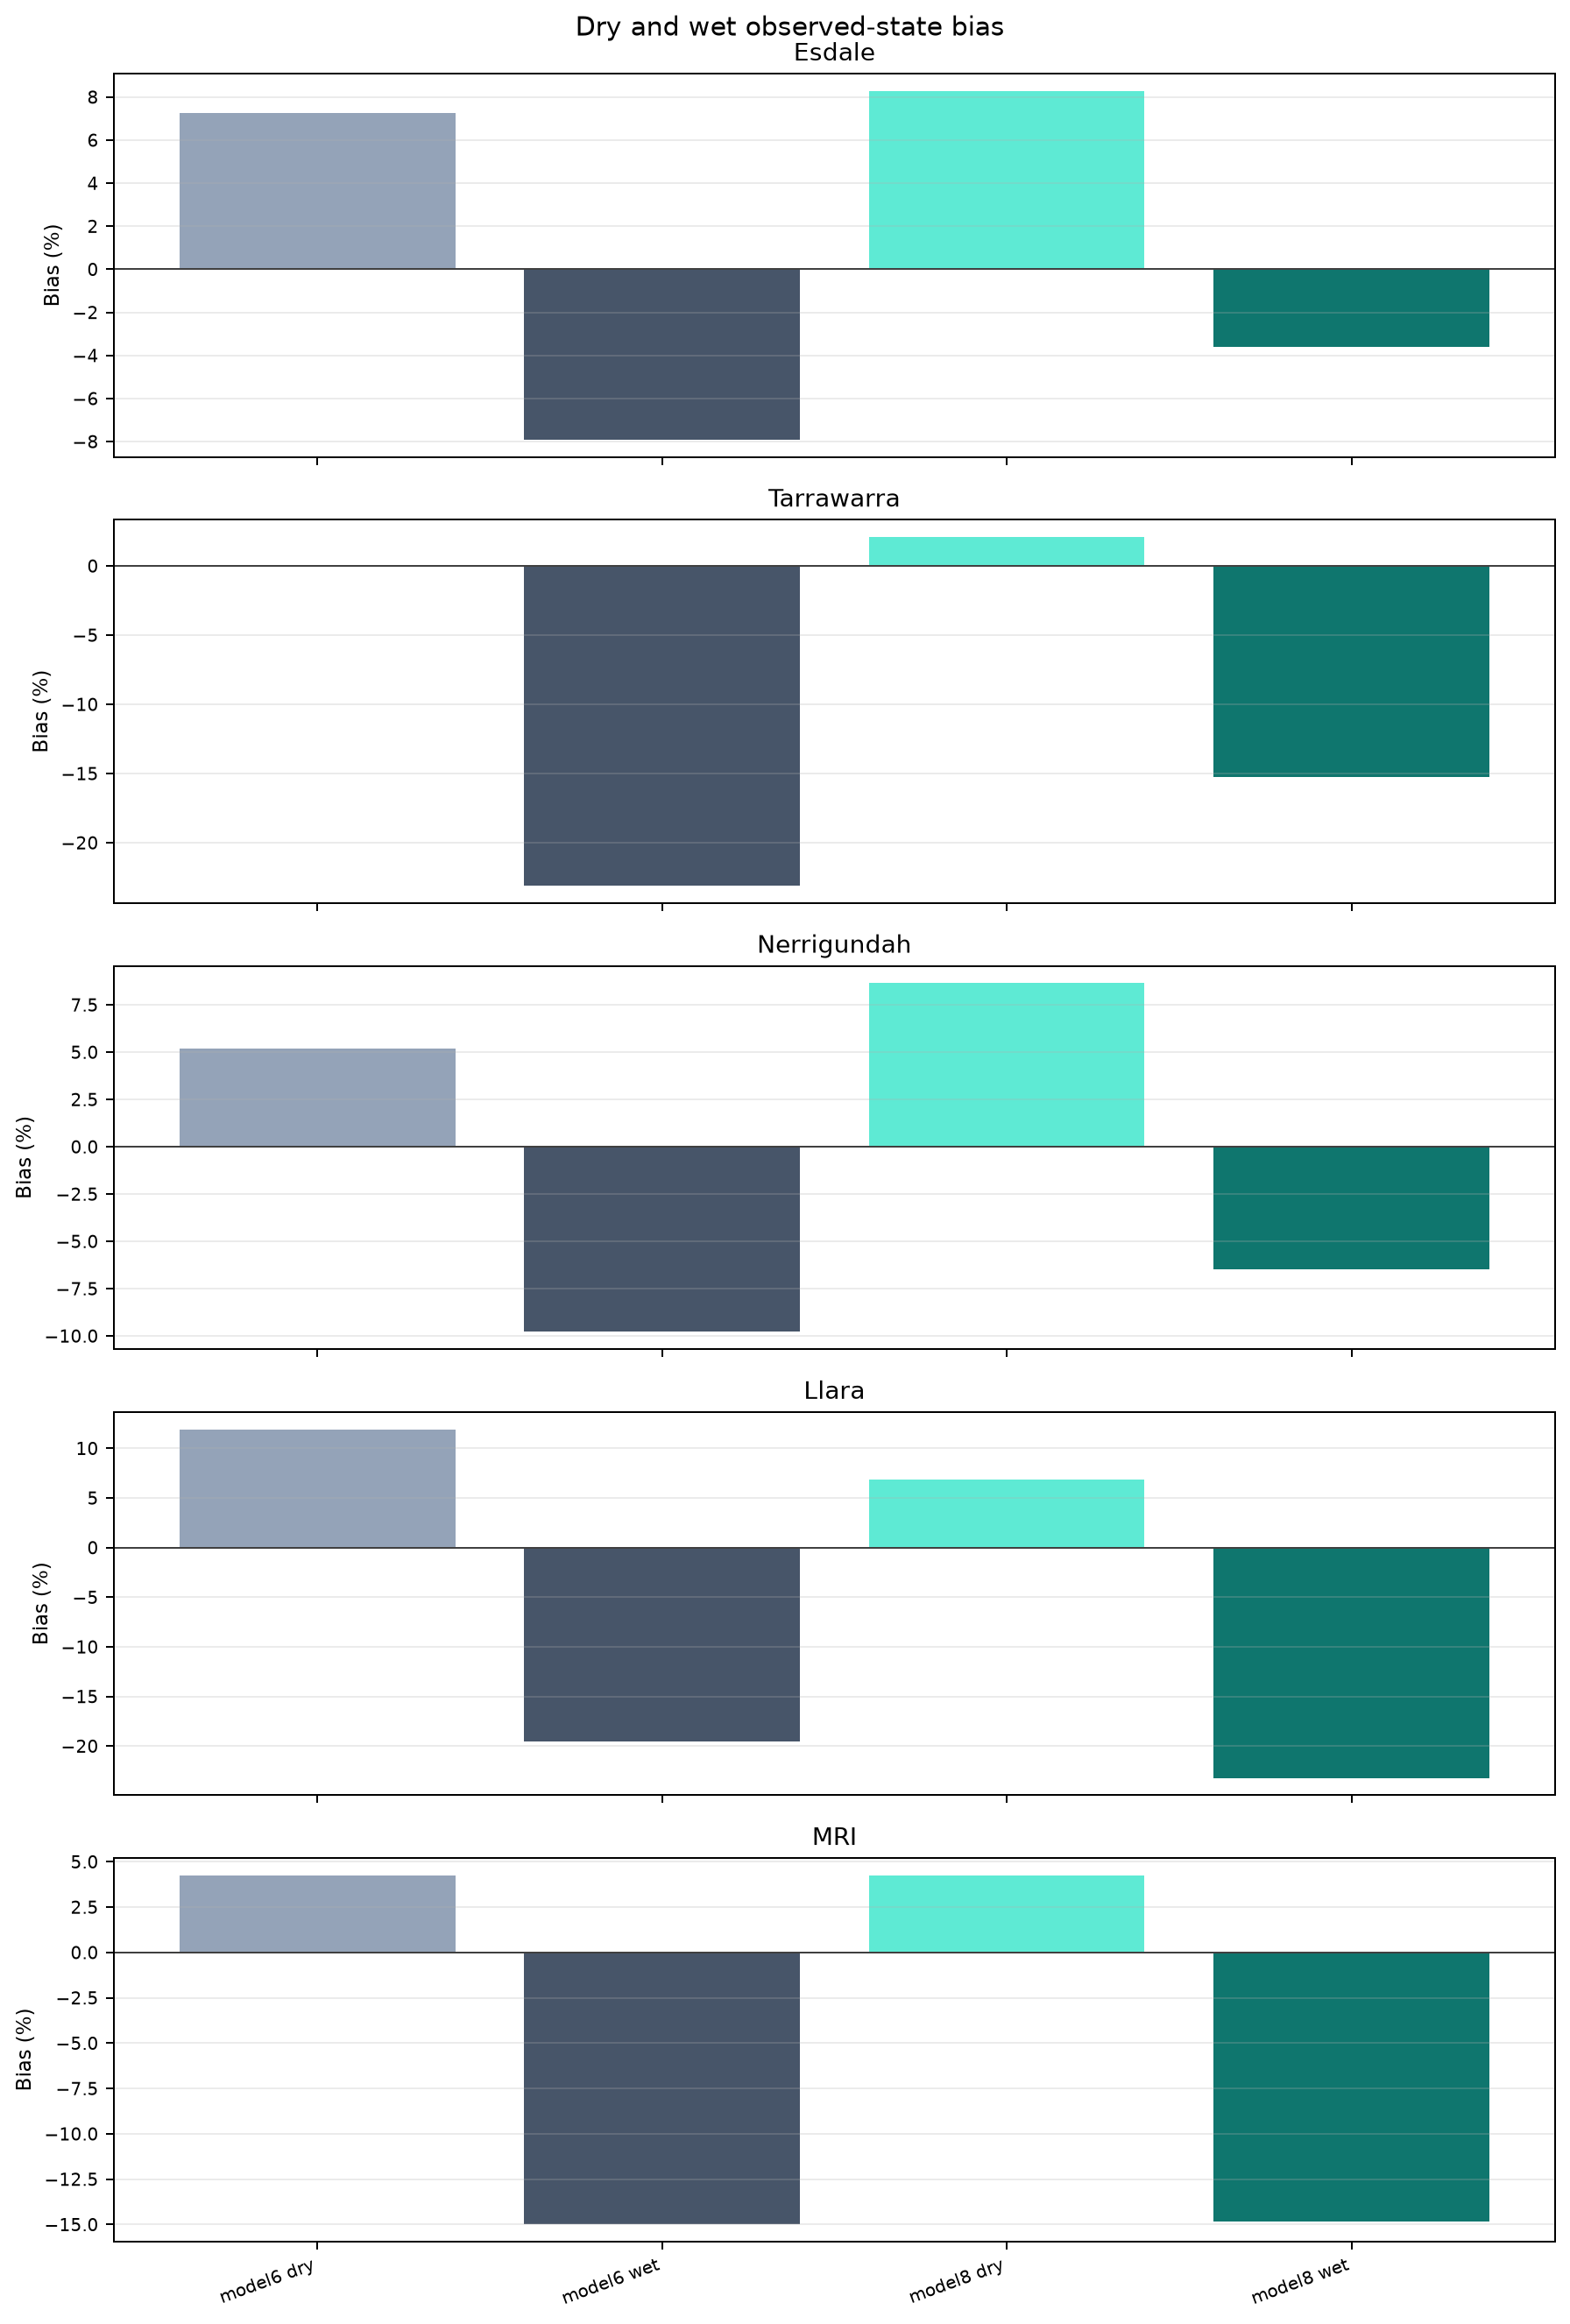
\includegraphics[width=0.92\textwidth]{wetness_quantile_bias.png}
\caption{Dry/wet observed-state bias.  The driest and wettest observed
quartiles test whether models compress extremes.  \todo{Add final interpretation:
overprediction in dry quartile, underprediction in wet quartile, or site/model
exceptions.}}
\label{fig:wetness-bias}
\end{figure}

\FloatBarrier

\subsection{Terrain and model-input stratification of error}
\label{sec:stage1-terrain}

The validation supports allow error to be stratified by the same model inputs
that drive the downscaling field, including elevation, slope, TWI, HLI,
accumulation, aspect components, SLGA soil properties and antecedent
meteorological summaries.  The main text should show only the most notable
strata; complete strata tables belong in the supplement.

To keep the terrain-space story simple, the manuscript version emphasises
support-level RMSE rather than showing both signed bias and RMSE in the same
section.  Each point in Figs.~\ref{fig:pca-static-global-rmse} and
\ref{fig:pca-static-site-rmse} is a validation support: an Esdale, Llara or MRI
probe location, or a Tarrawarra/Nerrigundah grid-cell support after campaign
aggregation.  The colour is the RMSE for that support pooled across available
dates, shown separately for \modelSix{} and \modelEight{}.

The global-scaled PCA asks whether the validation sites occupy different
absolute terrain--soil settings (Fig.~\ref{fig:pca-static-global-rmse}).  This
view preserves site means, so between-site separation should be interpreted as
environmental transfer distance.  High-RMSE clusters in this plot therefore
suggest that a model is failing in particular absolute terrain--soil
environments, but they may also reflect site-level offsets, sensor depth
differences or historical coarse-anchor caveats.

\begin{figure}[htbp]
\centering
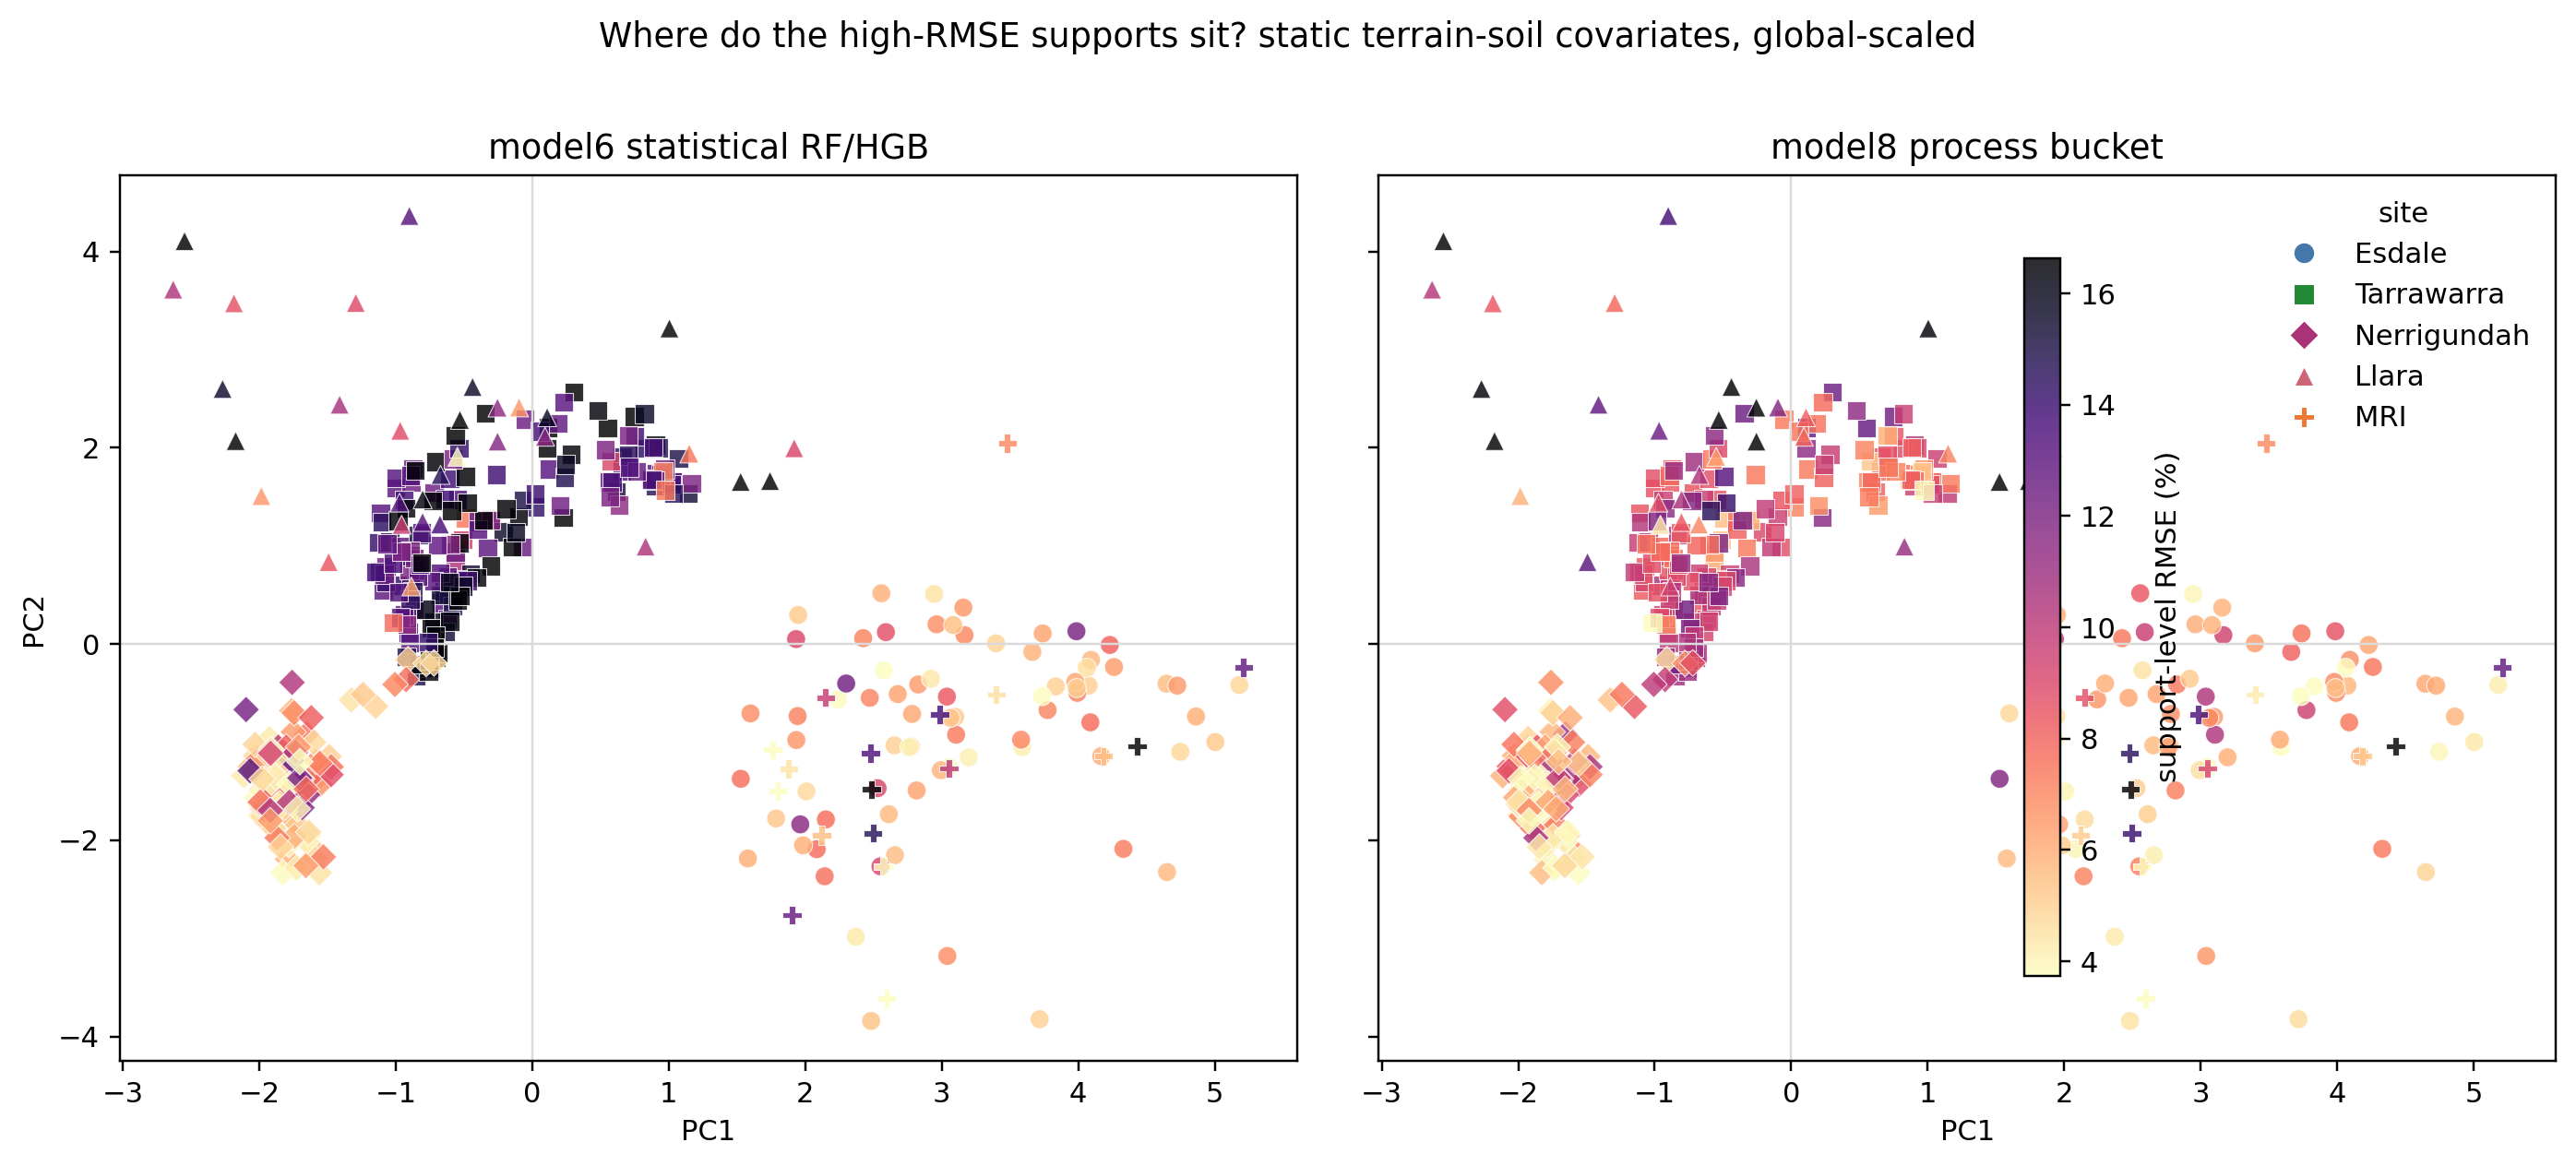
\includegraphics[width=\textwidth]{static_terrain_soil_global_rmse_pca.png}
\caption{Global-scaled static terrain--soil PCA with supports coloured by
support-level RMSE.  PCA inputs are elevation, slope, aspect components, TWI,
HLI, accumulation and SLGA soil properties.  The same support coordinates are
shown in both model panels; only the RMSE colouring differs.}
\label{fig:pca-static-global-rmse}
\end{figure}

The site-standardised PCA removes each site's mean terrain--soil offset before
fitting the PCA (Fig.~\ref{fig:pca-static-site-rmse}).  This is the cleaner
view for asking whether high-error supports occupy analogous within-site
positions, for example local ridges, hollows, high-HLI positions or soil-texture
extremes.  This view should be interpreted as a diagnostic map of terrain
failure modes, not as a causal attribution model; the PCA axes are rotations of
correlated covariates.

\begin{figure}[htbp]
\centering
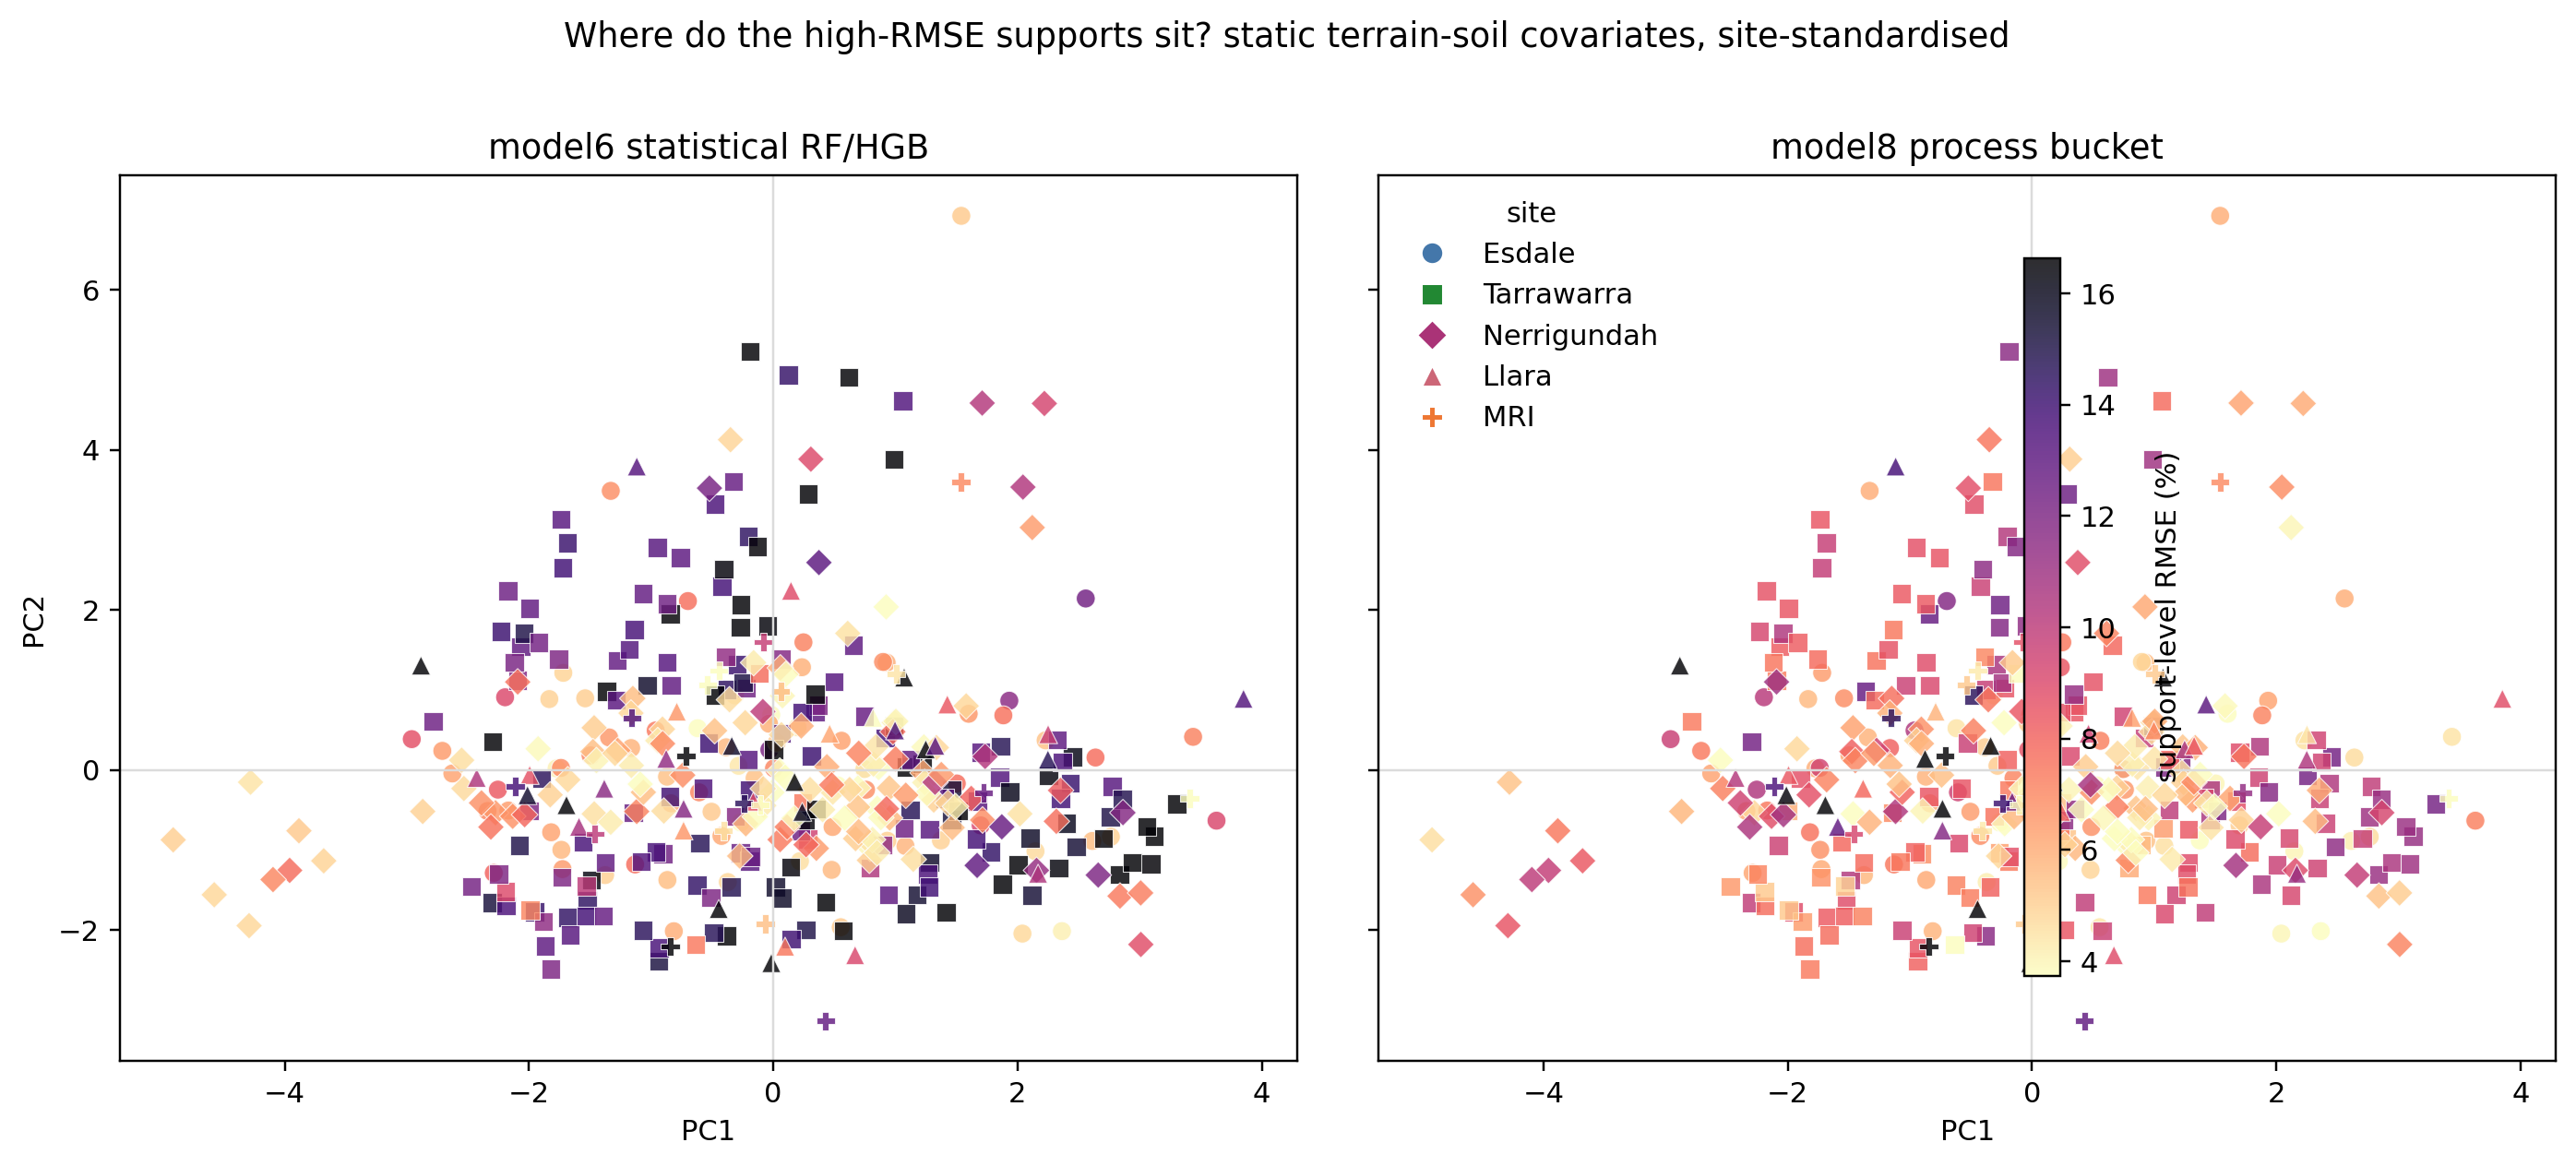
\includegraphics[width=\textwidth]{static_terrain_soil_site_standardised_rmse_pca.png}
\caption{Site-standardised static terrain--soil PCA with supports coloured by
support-level RMSE.  Within each site, static covariates are z-scored before
PCA, so local terrain contrasts are comparable across sites even when the
absolute site environments differ.}
\label{fig:pca-static-site-rmse}
\end{figure}

\todo{After final figure choice, write one compact paragraph naming the most
visible high-RMSE terrain-space regions and whether those regions are shared by
\modelSix{} and \modelEight{}.  Keep signed-bias PCA as supplementary unless it
adds a distinct manuscript claim.}

\subsection{Spatial clustering of prediction quality}
\label{sec:stage1-spatial}

Prediction-quality maps test whether poor performance is spatially organised.
For publication, show support-level maps of \nse{}, Pearson $\pearsonr$, RMSE,
\ubrmse{} and bias where sample size permits, plus a paired model-advantage map
where useful.  Interpolated quality surfaces can aid visual diagnosis but
should be labelled as diagnostic interpolation, not model output.

\begin{figure}[htbp]
\centering
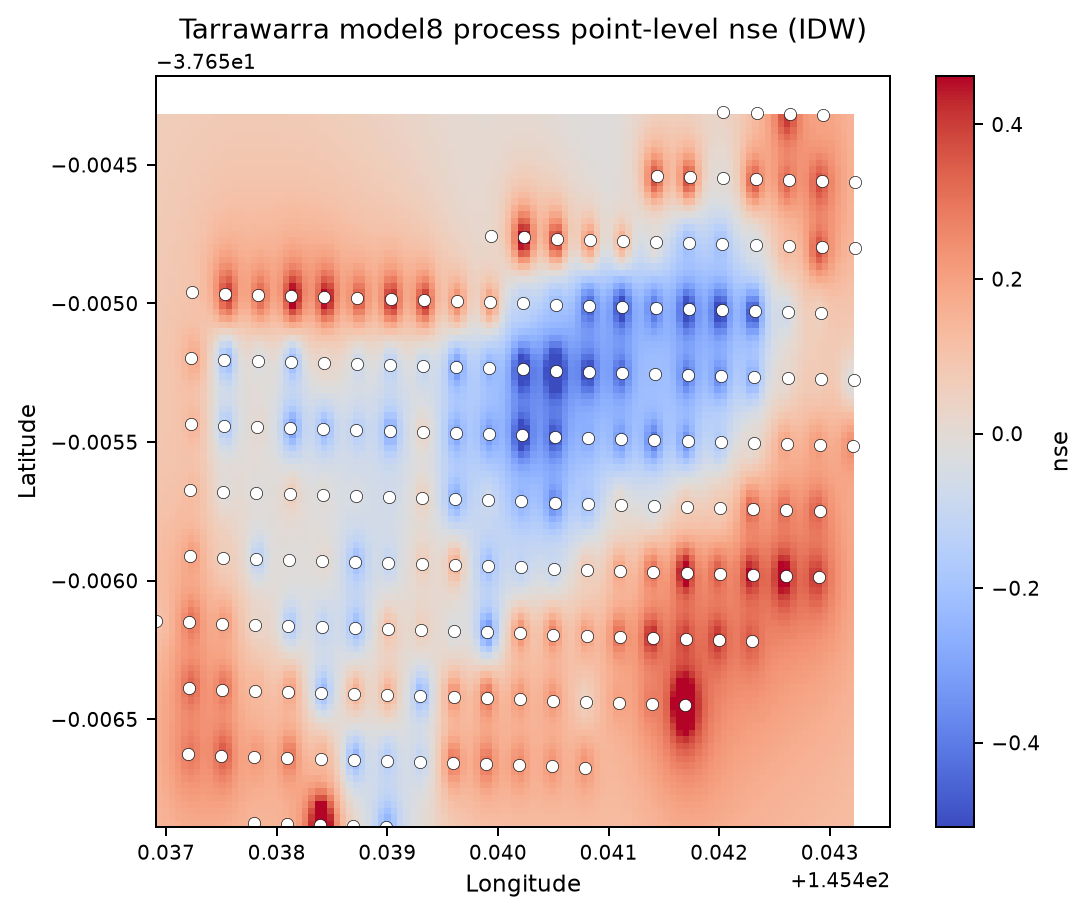
\includegraphics[width=0.32\textwidth]{tarrawarra_model8_process_nse_idw_surface.png}
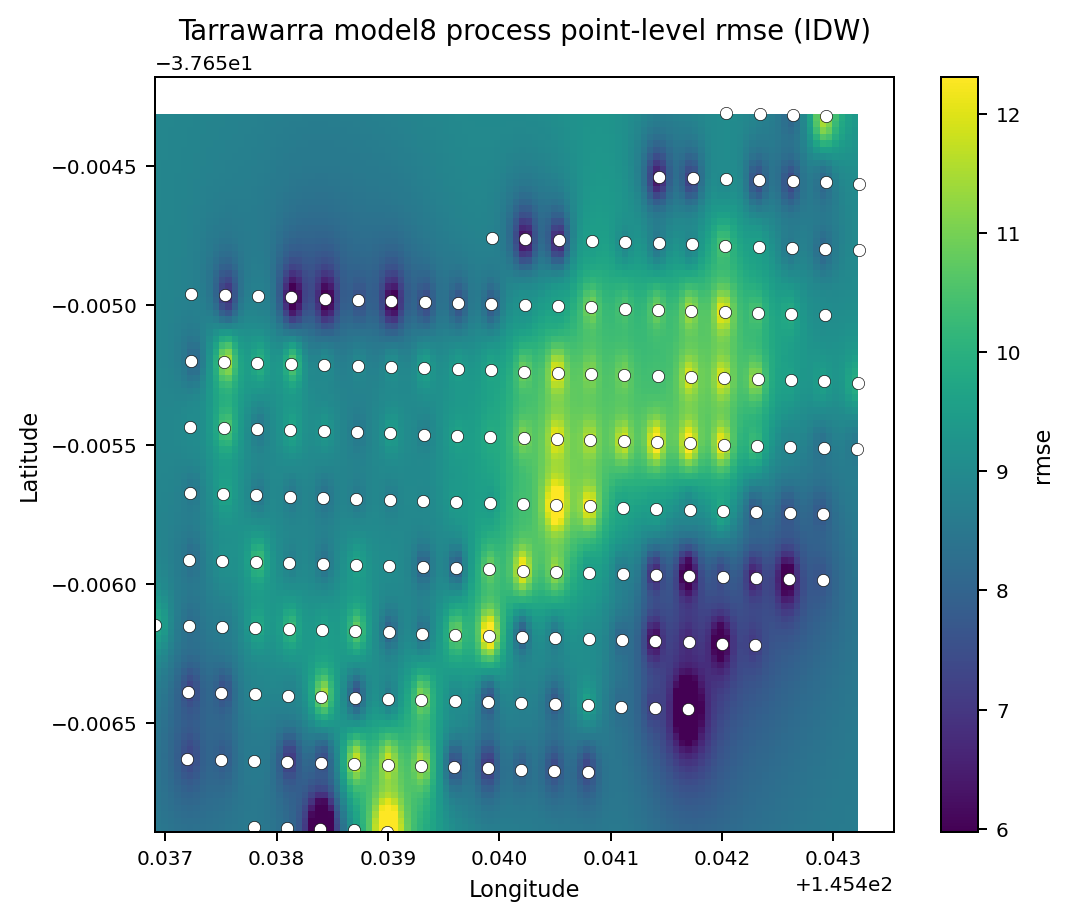
\includegraphics[width=0.32\textwidth]{tarrawarra_model8_process_rmse_idw_surface.png}
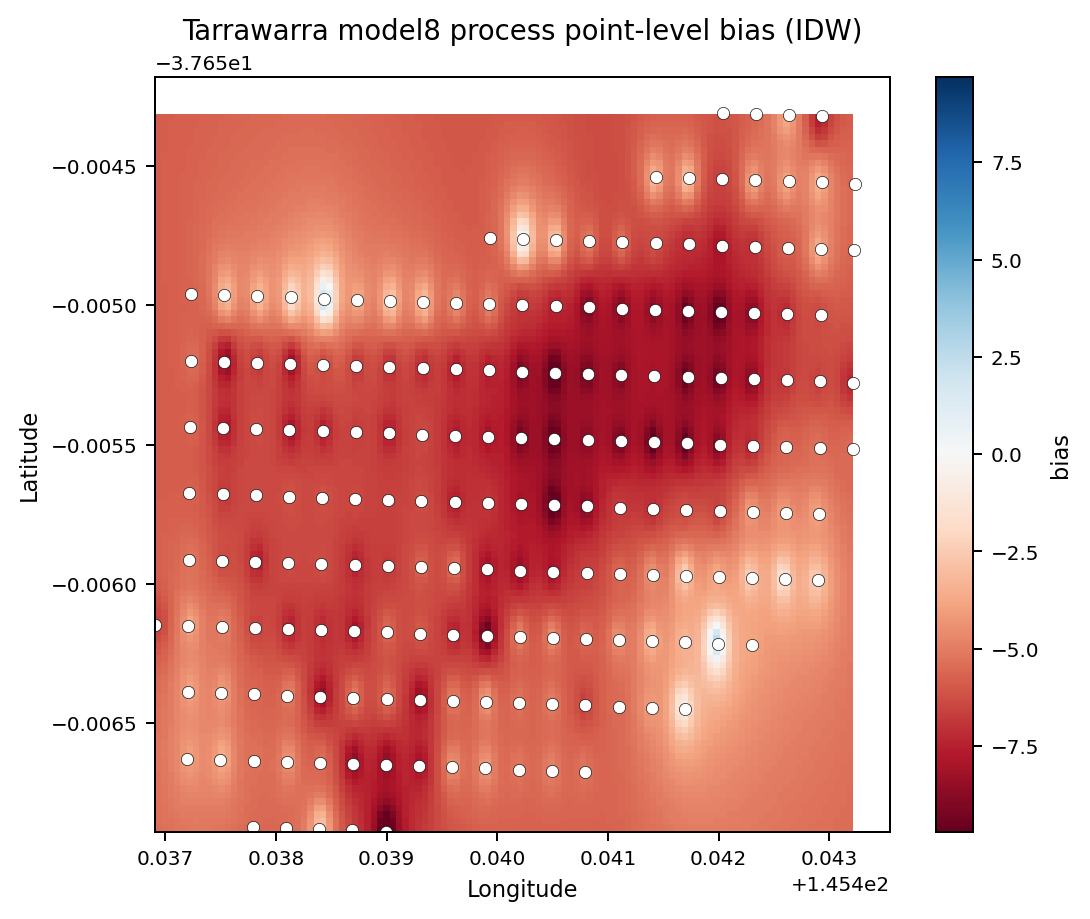
\includegraphics[width=0.32\textwidth]{tarrawarra_model8_process_bias_idw_surface.png}
\caption{Example spatial prediction-quality surfaces for Tarrawarra
\modelEight{}.  These are diagnostic interpolations of validation metrics at
aggregated model-grid-cell support, not gridded model predictions.  \todo{Replace
or extend with a final multi-site figure that uses consistent colour scales and
includes paired model-advantage maps.}}
\label{fig:quality-surfaces}
\end{figure}

\FloatBarrier

\section{Stage 2: sparse local calibration and local spiking}
\label{sec:stage2}

\subsection{Rationale}\label{sec:stage2-rationale}

Independent validation tells us where the national/global model fails.  A
deployment question follows: can a small amount of local information correct
site-level or terrain-conditioned bias without requiring dense sampling at
every property?  This stage should be interpreted as a local adaptation
experiment, not as independent validation of the base models.

The experiment should mimic realistic local information.  A new landholder
will usually not know where the model performs badly, but may know where the
landscape is generally wet, dry, low, high, clayey or exposed.  Calibration
point selection should therefore compare random selection against simple
landscape-knowledge proxies and model-informed extremes.

\subsection{Calibration layers and point-selection strategies}
\label{sec:stage2-methods}

The current calibration layers are:

\begin{enumerate}
\item \textbf{Bias offset:} one constant residual correction.
\item \textbf{Seasonal offset:} separate residual offsets by season where
  enough dates exist.
\item \textbf{Affine correction:} local linear rescaling of prediction level.
\item \textbf{Residual ridge layer:} residual model using selected model-input
  covariates.
\end{enumerate}

Point budgets are three, five, ten, 25\,\%, 50\,\% and all eligible local
calibration points.  Validation is performed on held-out points and dates, with
the strict spatial+temporal block treated as the primary transfer estimate.

\todo{State exactly which selection strategies are retained in the final
protocol.  Current set: random, landscape wet/dry prior, global-prediction
extremes, and the field-knowledge wet/dry proxy upper bound.}

\subsection{Learning curves}\label{sec:stage2-learning}

The learning curves summarise whether sparse local calibration improves
strictly held-out supports as more local information is supplied.  To match the
minimum-budget analysis in Table~\ref{tab:min-budget}, the main figures show
the best deployable non-random, non-proxy strategy at each point budget: either
the landscape wet/dry prior or global-prediction extremes, excluding the
observed wet/dry proxy.  RMSE gain is useful because it has the same units as
soil moisture (Fig.~\ref{fig:learning-curves-rmse}), but it can hide whether
the calibrated model becomes efficient relative to the observed variance.  The
corresponding \nse{} learning curve (Fig.~\ref{fig:learning-curves-nse})
therefore shows whether calibration moves the model toward modest but
interpretable efficiency thresholds such as \nse{} $\approx 0.2$--0.3.  Random
placement is retained as an appendix comparator because it was generally
ineffective under the strict block.

\begin{figure}[htbp]
\centering
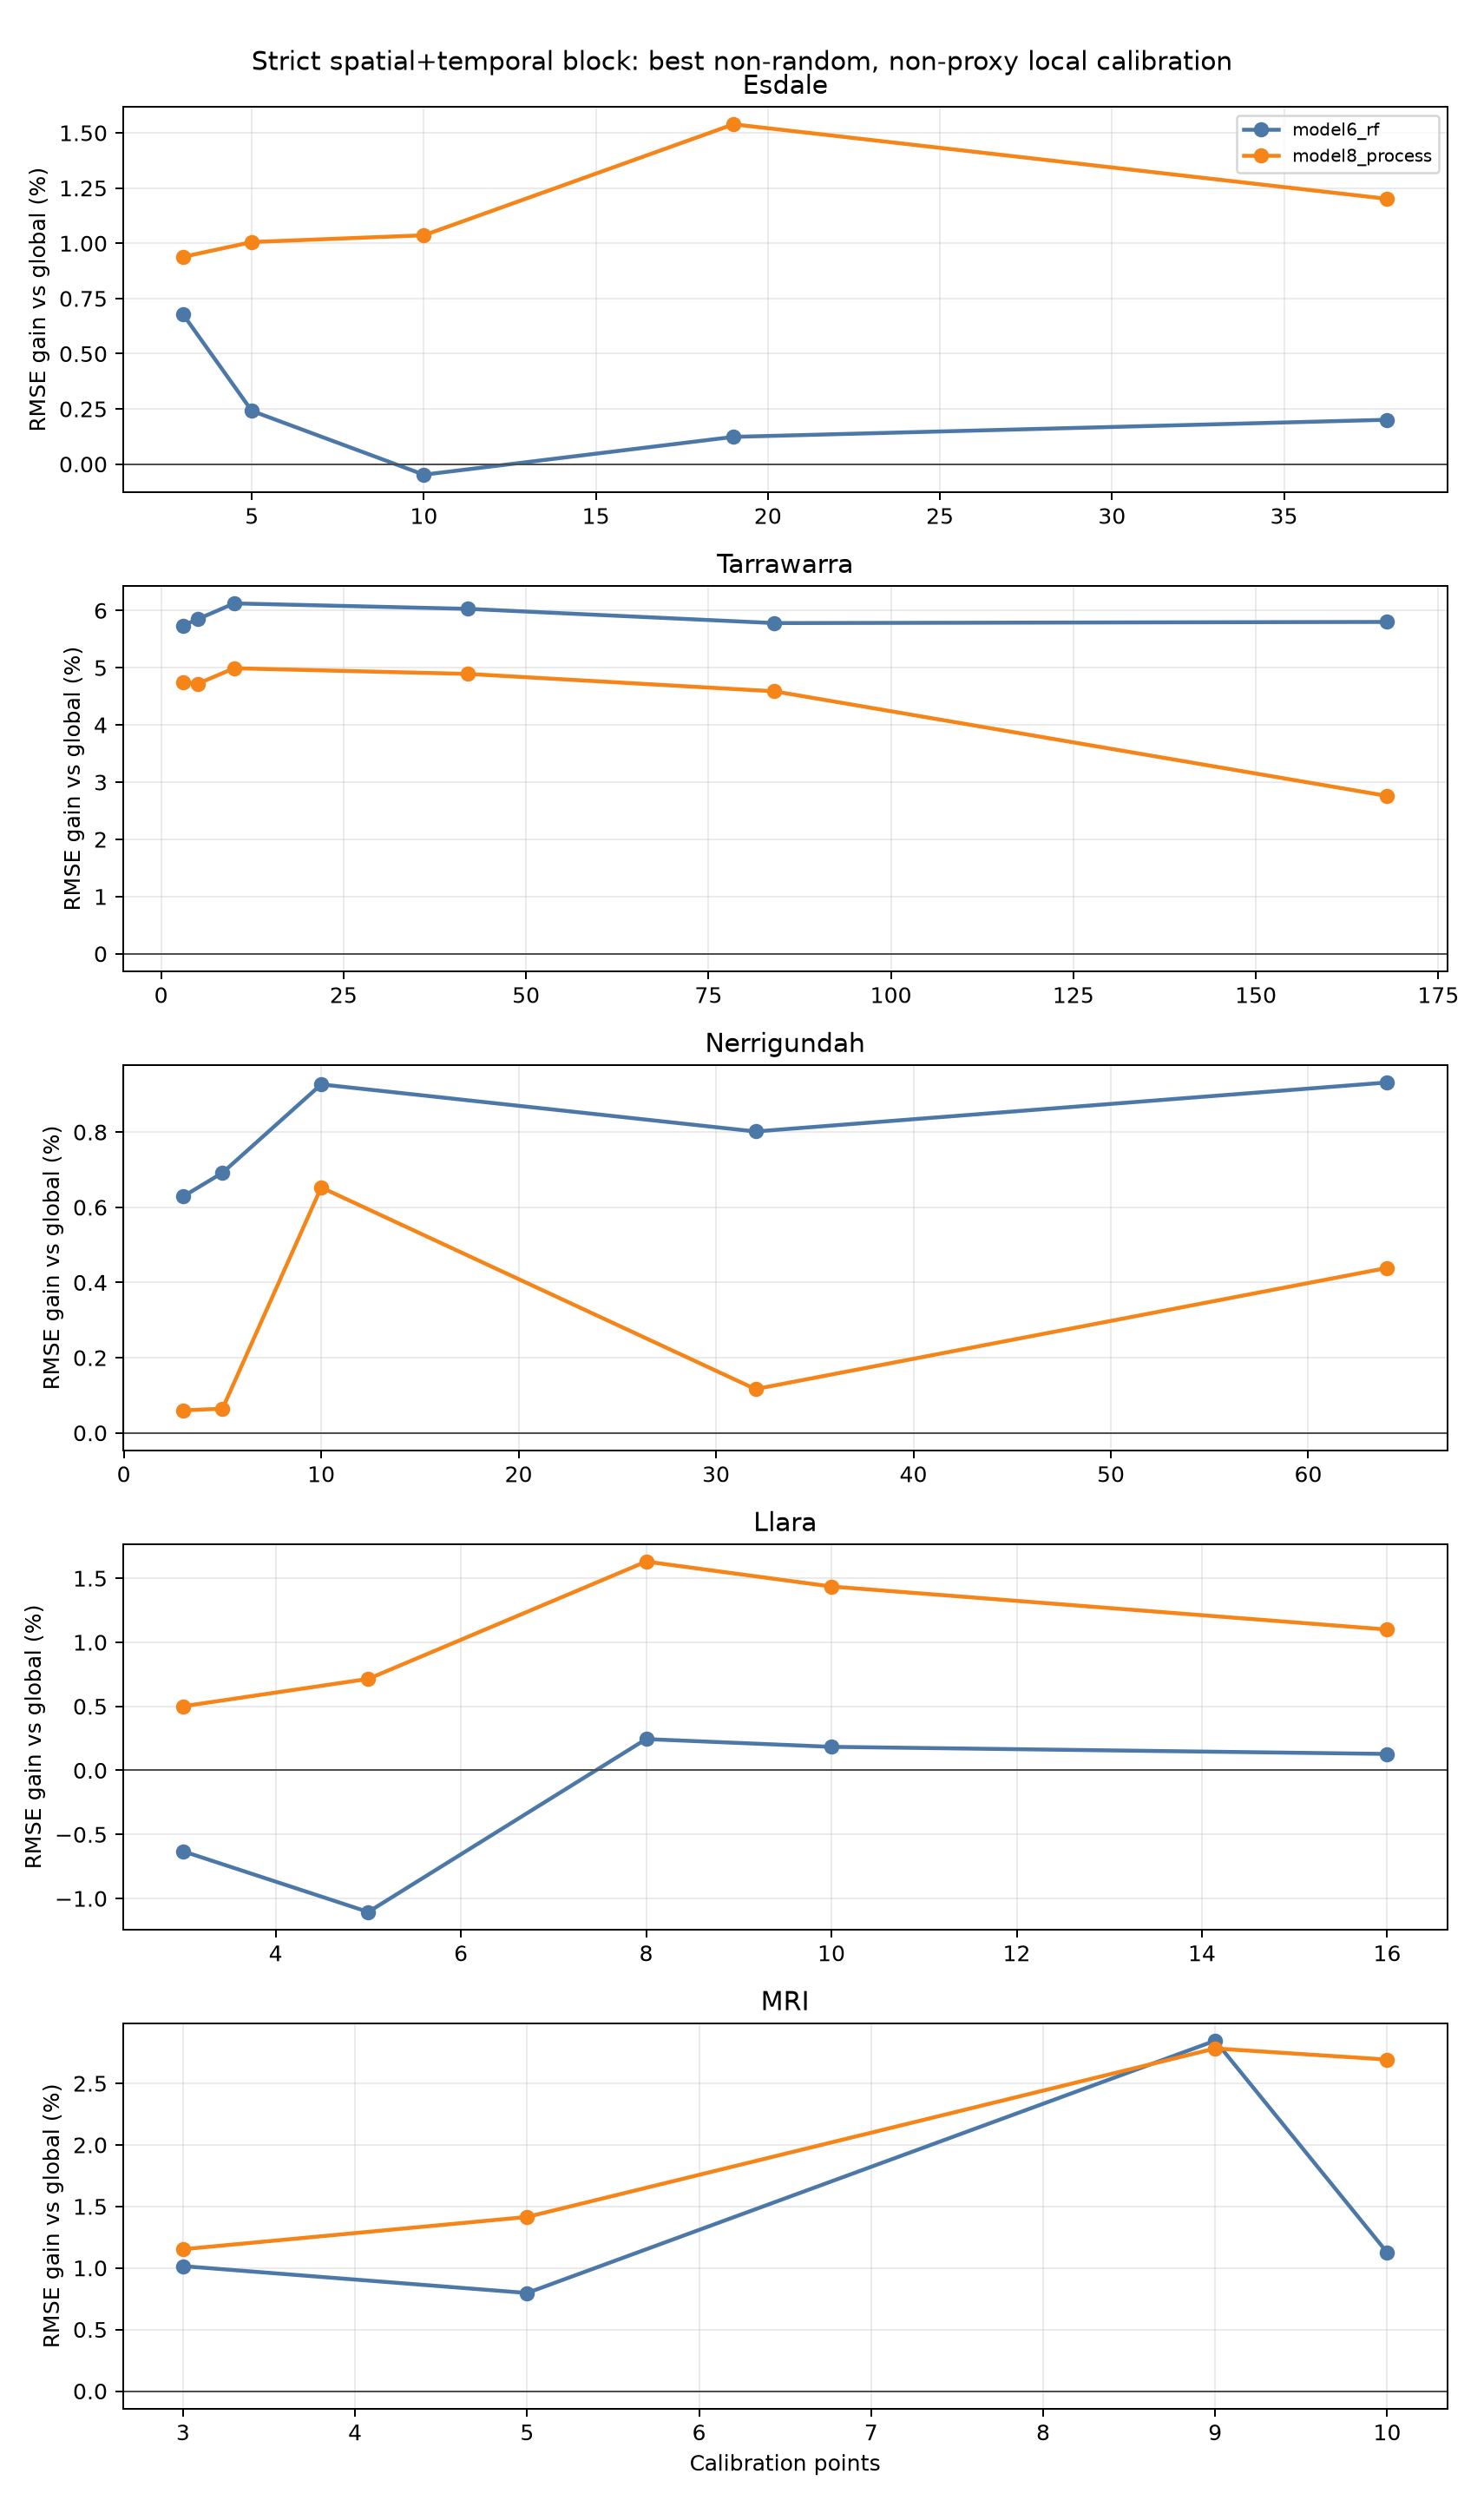
\includegraphics[width=\textwidth,height=0.82\textheight,keepaspectratio]{prior_guided_spatiotemporal_learning_curves_rmse_gain.png}
\caption{Prior-guided sparse local-calibration learning curves under strict
spatial+temporal blocking.  Each point is the best deployable non-random,
non-proxy strategy/method combination for that site, model and local point
budget.  Positive values indicate lower RMSE after calibration.}
\label{fig:learning-curves-rmse}
\end{figure}

\begin{figure}[htbp]
\centering
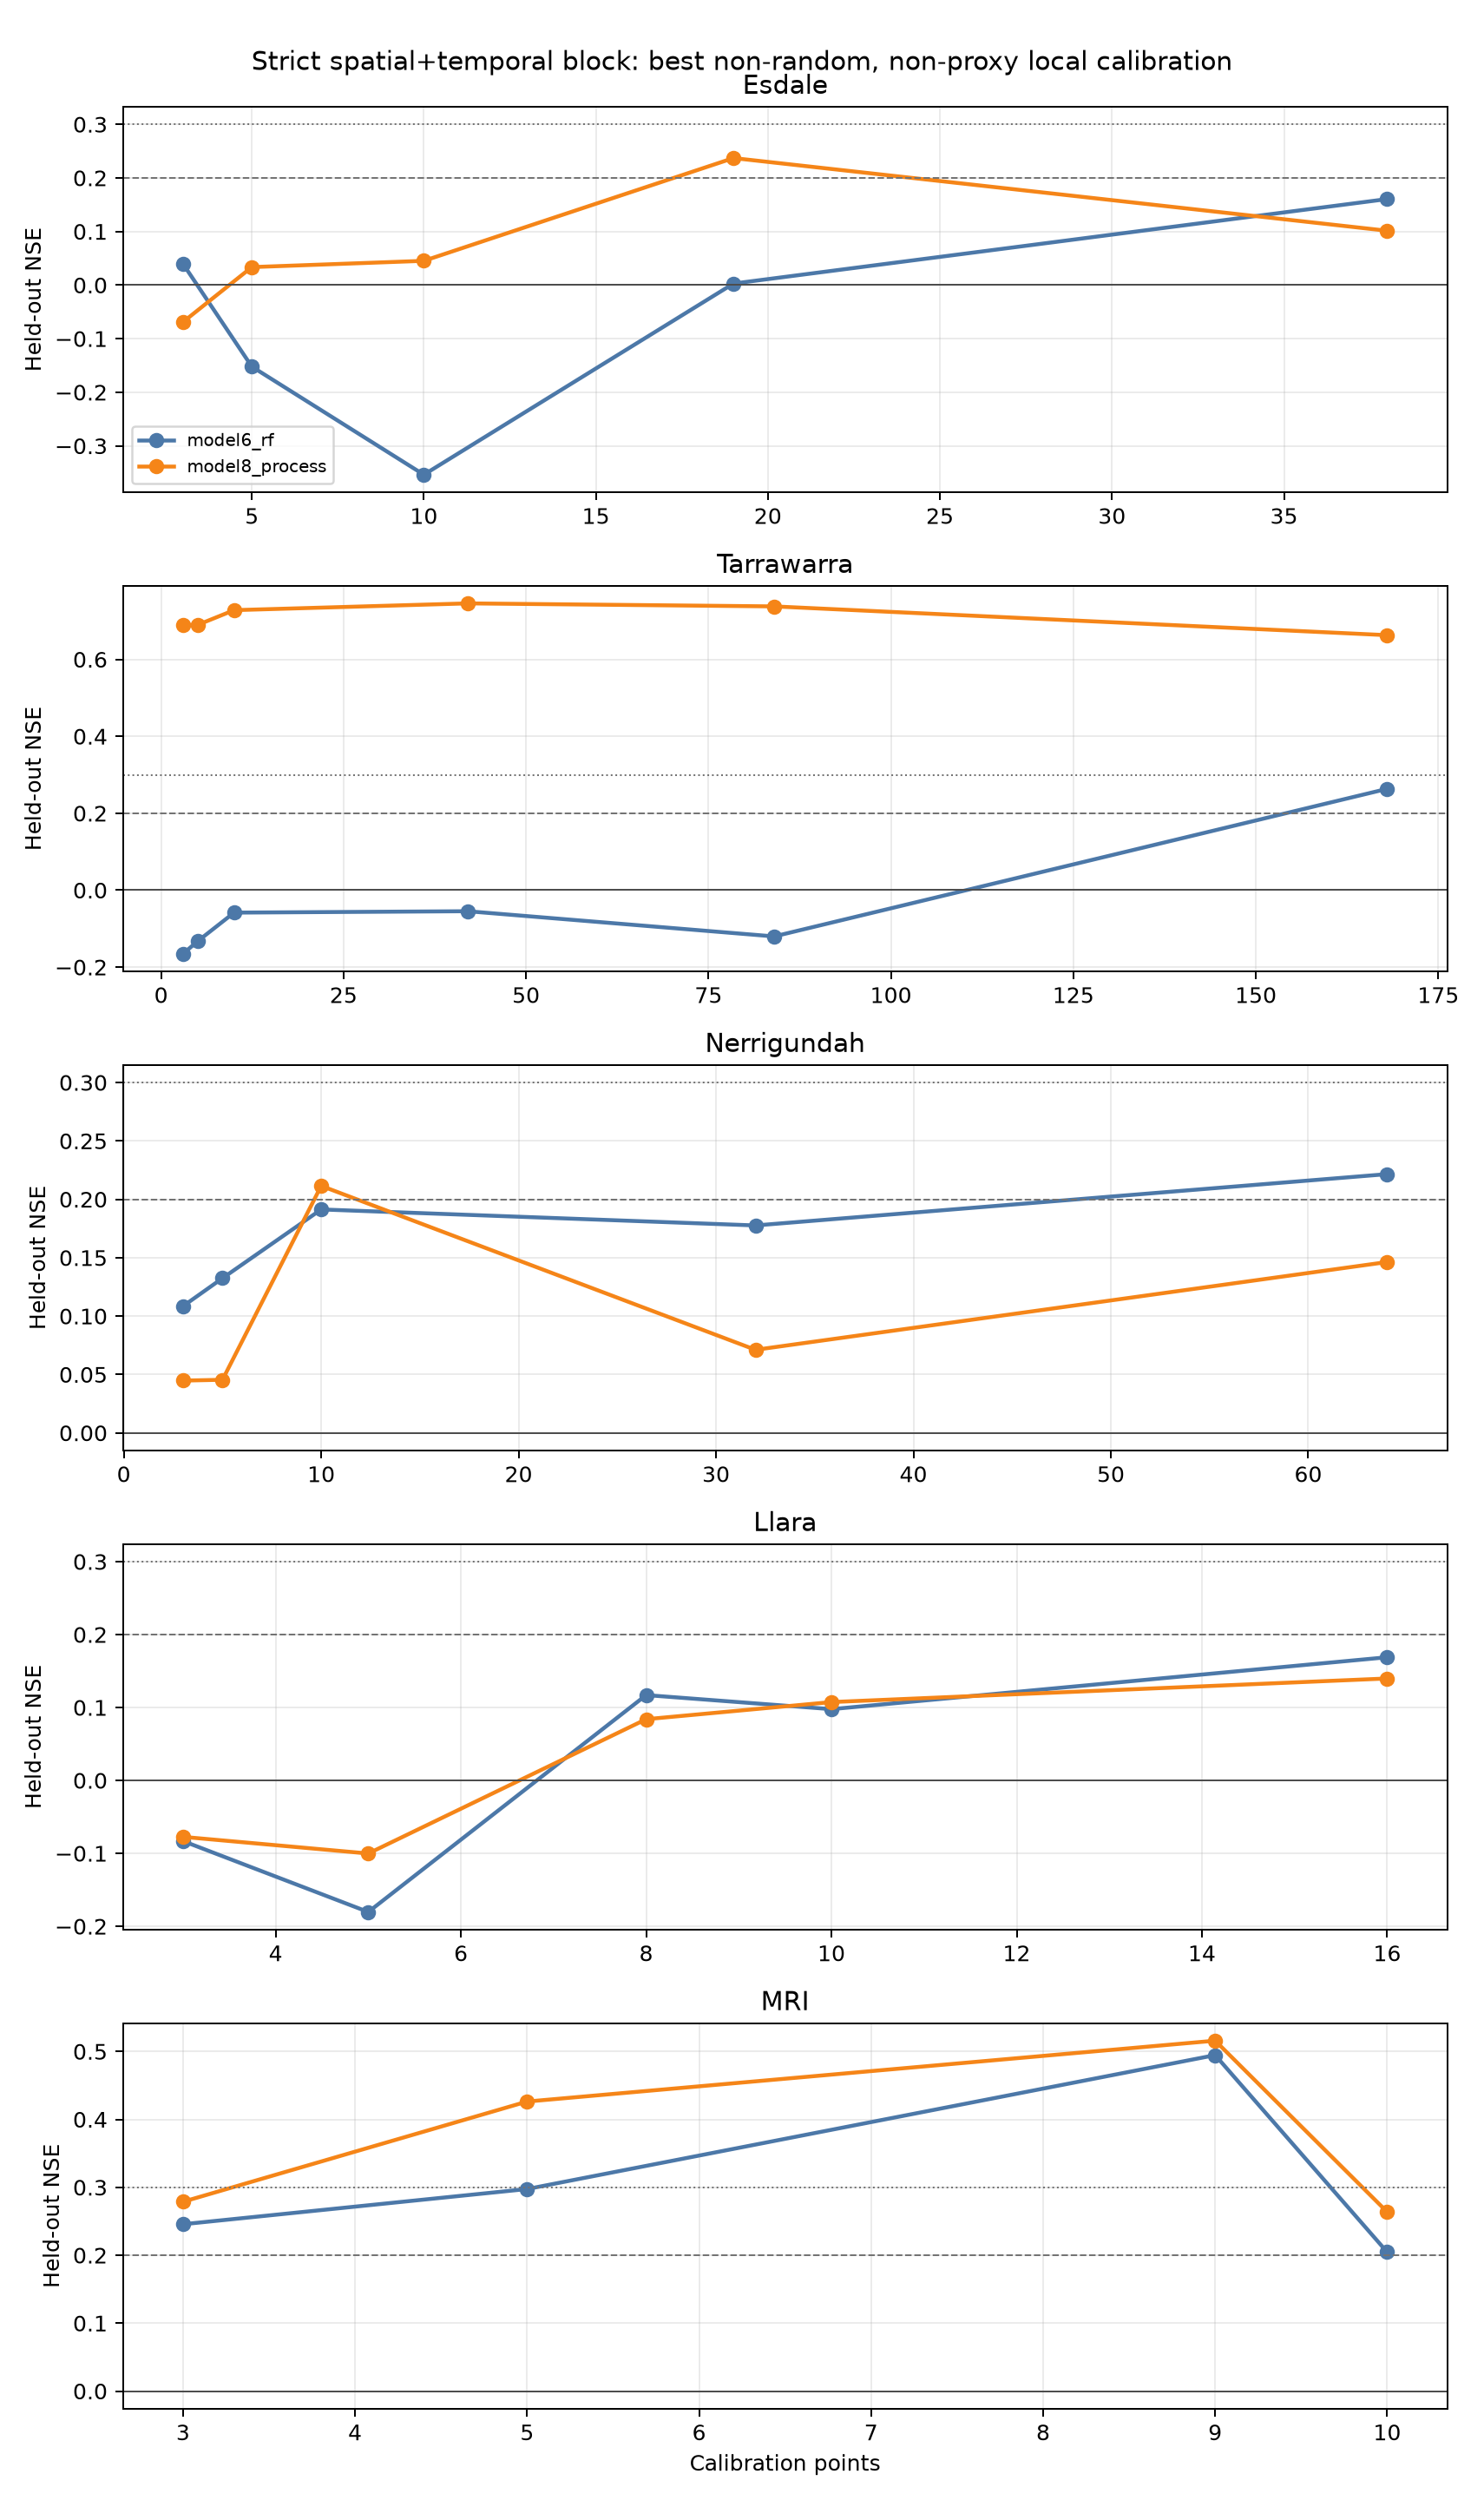
\includegraphics[width=\textwidth,height=0.82\textheight,keepaspectratio]{prior_guided_spatiotemporal_learning_curves_nse.png}
\caption{Prior-guided sparse local-calibration learning curves expressed as
held-out \nse{} under strict spatial+temporal blocking.  Each point is selected
using the same deployable non-random, non-proxy strategy set as
Table~\ref{tab:min-budget}.  Dashed and dotted reference lines mark
\nse{} = 0.2 and 0.3, respectively.  These thresholds are not universal
performance targets, but they are useful for asking how much local information
is needed before calibration becomes meaningfully better than the uncalibrated
baseline.}
\label{fig:learning-curves-nse}
\end{figure}

\FloatBarrier

\subsection{Minimum local information budgets}\label{sec:stage2-minimum-budget}

The deployment question is framed as a minimum information budget: how many
local supports are needed before strict held-out \nse{} reaches approximately
0.2 or 0.3?  Table~\ref{tab:min-budget} uses the current strict
spatial+temporal block and excludes the
\texttt{field\_knowledge\_wetdry\_proxy} upper-bound strategy because that
proxy uses observed chronic wet/dry behaviour.  The result is mixed rather than
uniformly optimistic.  Tarrawarra \modelEight{} responds strongly with three
landscape-prior supports, MRI reaches \nse{} = 0.3 with five to nine supports,
and Nerrigundah reaches \nse{} = 0.2 but not 0.3.  Esdale \modelSix{} and both
Llara models remain below 0.2 under the deployable prior-guided designs in this
cache.  The practical sensor-placement story should therefore emphasise
parsimonious but defensible local information budgets, not the assumption that
any small sensor set will fix within-property failure modes.

\begin{table}[htbp]
\centering
\small
\caption{Minimum local calibration supports needed to reach modest held-out
\nse{} thresholds under the strict spatial+temporal block.  Entries report the
smallest non-proxy strategy/method combination reaching the threshold, or the
best current result if the threshold is not reached.}
\label{tab:min-budget}
\begin{tabularx}{\textwidth}{llXX}
\toprule
Site & Model & \nse{} $\geq 0.2$ & \nse{} $\geq 0.3$ \\
\midrule
Esdale & \modelSix{} &
Not reached; best 38 supports, global-prediction extremes + residual ridge
(\nse{} = 0.160). &
Not reached; same best design (\nse{} = 0.160). \\
Esdale & \modelEight{} &
19 supports, landscape wet/dry prior + residual ridge (\nse{} = 0.237). &
Not reached; best \nse{} = 0.237. \\
Tarrawarra & \modelSix{} &
168 supports, global-prediction extremes + residual ridge (\nse{} = 0.263). &
Not reached; best \nse{} = 0.263. \\
Tarrawarra & \modelEight{} &
3 supports, landscape wet/dry prior + affine correction (\nse{} = 0.689). &
3 supports, landscape wet/dry prior + affine correction (\nse{} = 0.689). \\
Nerrigundah & \modelSix{} &
64 supports, landscape wet/dry prior + residual ridge (\nse{} = 0.222). &
Not reached; best \nse{} = 0.222. \\
Nerrigundah & \modelEight{} &
10 supports, landscape wet/dry prior + residual ridge (\nse{} = 0.211). &
Not reached; best \nse{} = 0.211. \\
Llara & \modelSix{} &
Not reached; best 16 supports, global-prediction extremes + bias offset
(\nse{} = 0.169). &
Not reached; same best design (\nse{} = 0.169). \\
Llara & \modelEight{} &
Not reached; best 16 supports, global-prediction extremes + bias offset
(\nse{} = 0.140). &
Not reached; same best design (\nse{} = 0.140). \\
MRI & \modelSix{} &
3 supports, global-prediction extremes + bias offset (\nse{} = 0.246). &
9 supports, global-prediction extremes + residual ridge (\nse{} = 0.495). \\
MRI & \modelEight{} &
3 supports, global-prediction extremes + bias offset (\nse{} = 0.279). &
5 supports, global-prediction extremes + residual ridge (\nse{} = 0.426). \\
\bottomrule
\end{tabularx}
\end{table}

\subsection{Do process and statistical models respond differently?}
\label{sec:stage2-process-vs-statistical}

The process-vs-statistical comparison is both technical and philosophical.  A
statistical downscaler may already encode nonlinear terrain and soil
relationships learned from the station network, but it may be brittle outside
the training distribution.  A process model may have simpler temporal dynamics
and fewer degrees of freedom, but a local layer may correct its site-level
state more cleanly.  The validation datasets allow this difference to be
measured as the marginal gain from the same sparse local information.

In the current strict prior-guided experiment, process-vs-statistical
responsiveness is site dependent rather than a single model ranking
(Fig.~\ref{fig:process-response}).  \modelEight{} often gains more than
\modelSix{} at Esdale and Llara, while Nerrigundah tends to favour larger gains
for \modelSix{} and MRI is mixed.  Tarrawarra remains a special case:
\modelSix{} begins with a large dry bias linked to the historical coarse-anchor
problem, so simple local calibration can remove part of that offset even when
\modelEight{} remains the lower-error model after calibration.  A clearer
mechanistic interpretation will require comparing the calibration supports
against model-input diagnostics such as TWI, HLI, elevation, soil texture,
antecedent rainfall/PET and the availability or failure mode of SMIPS/process
state variables.

\begin{figure}[htbp]
\centering
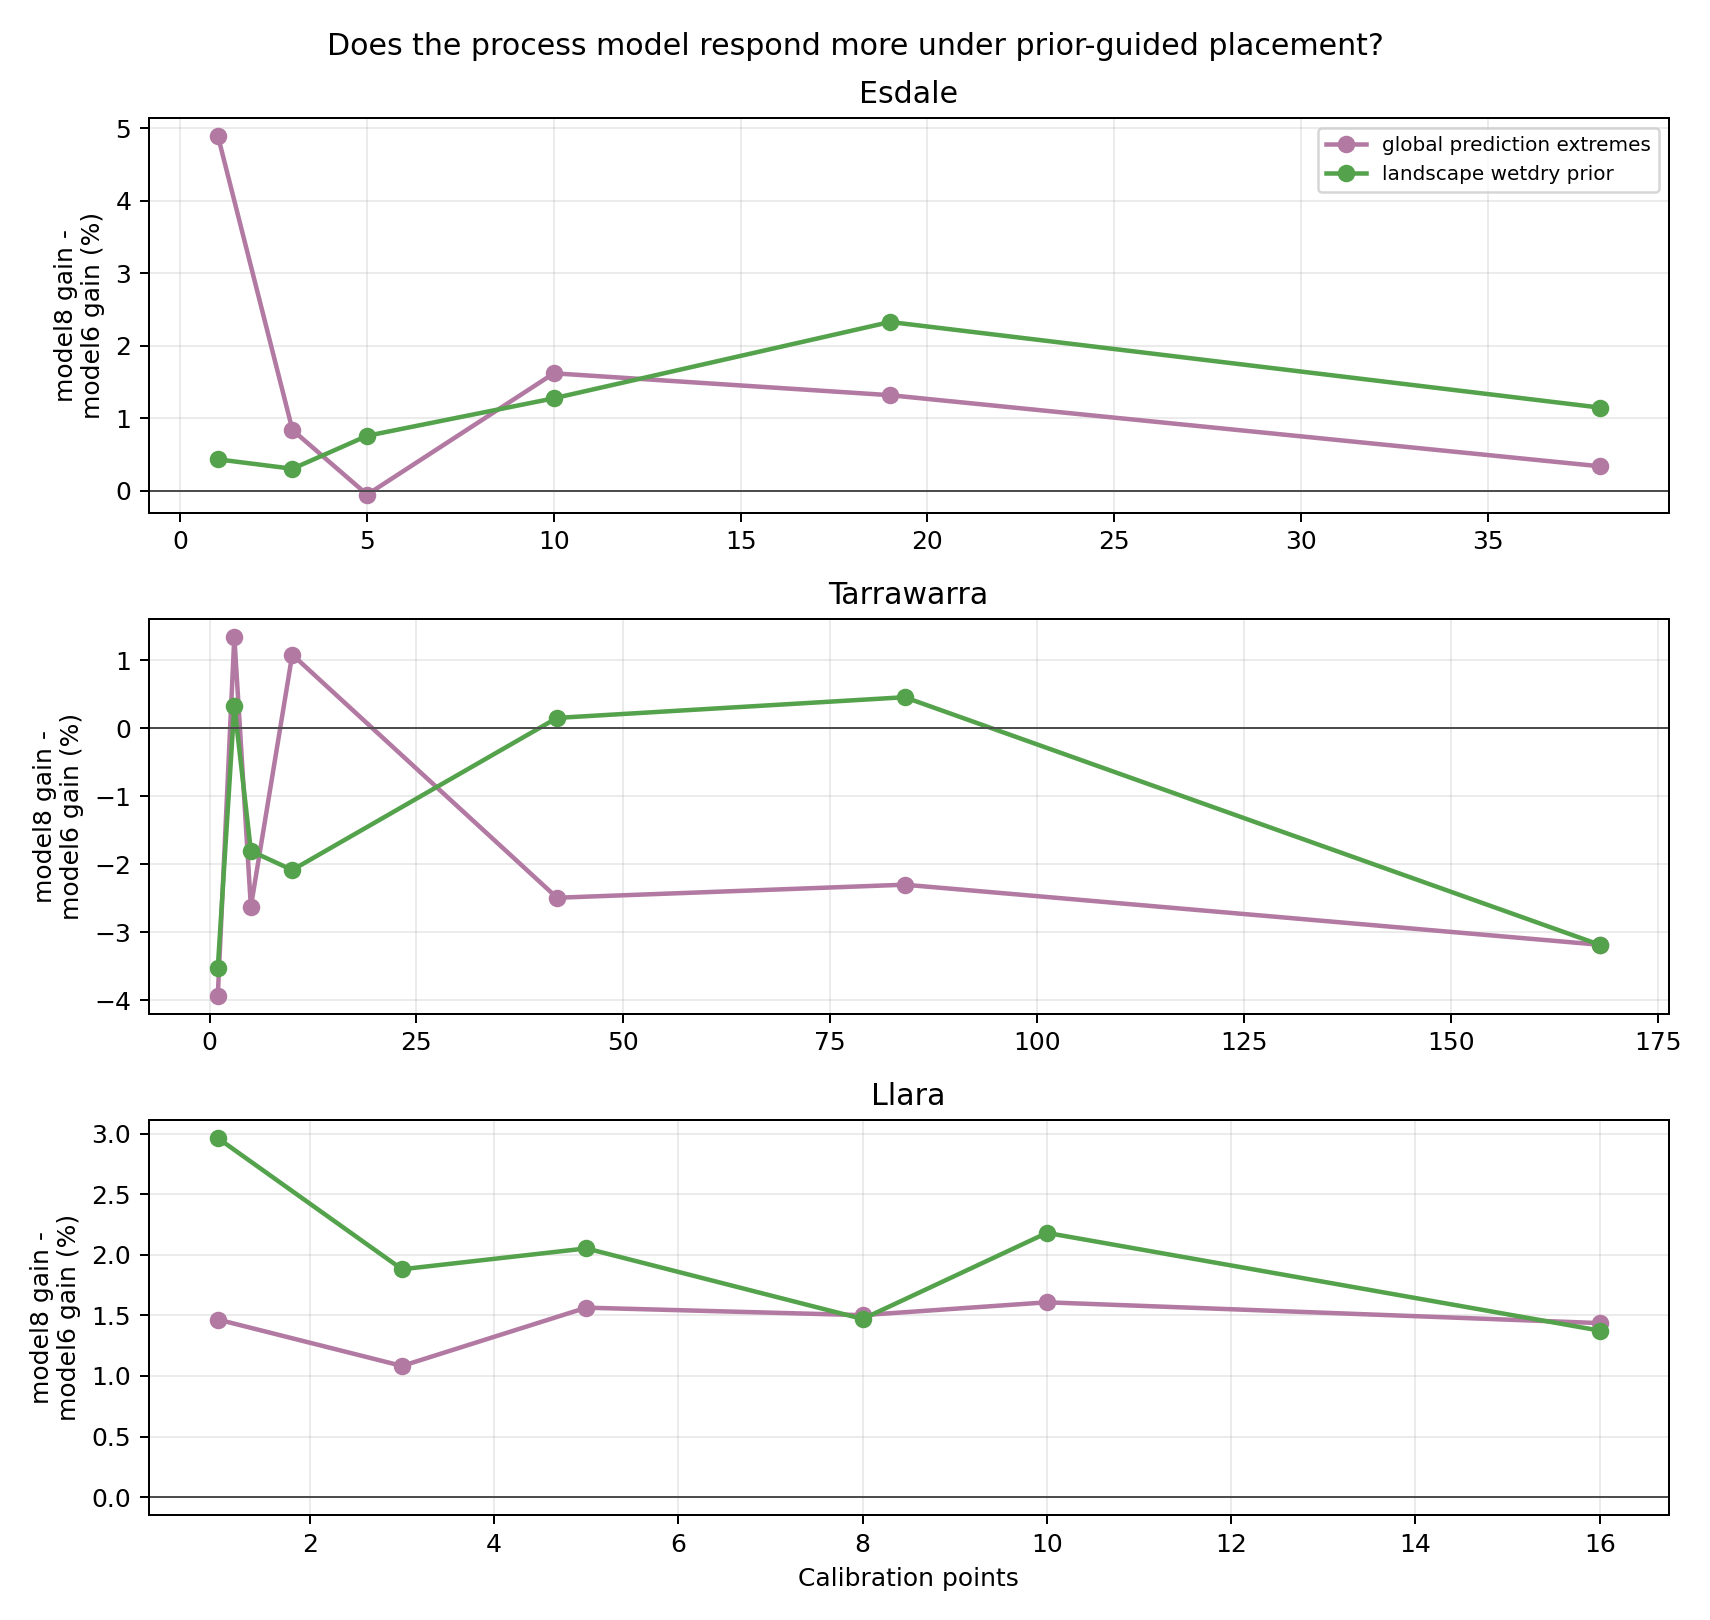
\includegraphics[width=0.9\textwidth,height=0.82\textheight,keepaspectratio]{prior_guided_process_vs_statistical_responsiveness.png}
\caption{Process-vs-statistical local calibration responsiveness under
deployable prior-guided placement.  Positive values indicate that
\modelEight{} gained more RMSE improvement than \modelSix{} from the same
non-random placement strategy and sparse local information budget under strict
spatial+temporal blocking.}
\label{fig:process-response}
\end{figure}

\FloatBarrier

\section{Discussion}\label{sec:discussion}

\subsection{What dense validation adds beyond station validation}
\label{sec:dense-adds}

\todo{Synthesis paragraph.  Suggested claim: the companion paper establishes
regional/station transfer; dense validation reveals whether the 30\,m product
has meaningful within-site spatial structure and whether residuals organise by
terrain, season and wetness state.}

\subsection{Model complementarity at paddock scale}
\label{sec:model-complementarity}

\todo{Discuss whether \modelSix{} and \modelEight{} fail in the same places.
Use paired comparisons and maps.  Avoid a single global winner unless the
paired evidence is strong and caveats are resolved.}

\subsection{Implications for local deployment}
\label{sec:deployment}

\todo{Discuss the sparse-sensor deployment story.  Frame local calibration as a
separate adaptation layer placed on top of a national/global model, not as
leakage into independent validation.}

\subsection{Future public training and validation data}
\label{sec:future-data}

\todo{Discuss likely value of additional public dense datasets, sensor
networks, campaign data and remote/proximal sensing products.  Separate data
that improve model training from data that improve independent validation.}

\section{Limitations}\label{sec:limitations}

\begin{itemize}
\item Esdale has strong spatial/terrain coverage but short autumn--winter
coverage.
\item Tarrawarra and Nerrigundah have exceptional raw point density; validation
now aggregates those points to model grid cells by date before scoring. Their
current \modelSix{} \smips{}-zero/coarse-anchor caveat prevents direct
interpretation as operational \modelSix{} performance. High within-cell TDR
variance should be treated as support mismatch unless future models explicitly
represent sub-pixel structure.
\item Llara has strong temporal/seasonal coverage but only 32 probes across
two paddocks.
\item MRI has a long continuous record but only 18 retained probe supports, so
its local-calibration results are sensitive to sparse-network geometry.
\item Soil-moisture depth definitions and profile integration differ across
datasets and must be documented carefully.
\item The validation datasets remain limited in climate and soil coverage
relative to the intended national product.
\item \nse{} can be unstable when observed variance is small; Pearson
$\pearsonr$, RMSE, \ubrmse{} and bias must be interpreted alongside it.
\item Local calibration experiments are deployment sensitivity analyses, not
independent validation of the base models.
\end{itemize}

\section{Conclusions}\label{sec:conclusions}

\todo{Write as 4--6 numbered conclusions.  Suggested structure:
(1) dense validation is a distinct evidence layer; (2) headline independent
skill and caveats; (3) seasonal/wetness/terrain bias; (4) model6/model8
complementarity; (5) sparse local calibration implications; (6) priority next
data.}

\section*{Code and data availability}

All validation code and report-generation scripts are maintained in the
\texttt{DMM\_validation} repository.  Model definitions and the companion paper
are maintained in the \texttt{DownscalingMoistureModel} repository.
\todo{Add repository URLs, branch names, commit hashes, data access statements
and any restrictions before submission.}

\section*{Supplementary material plan}

\begin{itemize}
\item Full model-agnostic prediction tables for Esdale, Tarrawarra,
Nerrigundah, Llara and MRI.
\item Full per-site/model metric tables.
\item Full terrain/model-input strata tables.
\item Full paired support/date model comparison tables.
\item Local calibration design tables, selected calibration points and
  replicate-level learning-curve outputs.
\item Additional prediction-quality maps and gridded dry/wet map examples.
\end{itemize}

\appendix
\renewcommand{\thefigure}{A\arabic{figure}}
\renewcommand{\theHfigure}{appendix.\arabic{figure}}
\setcounter{figure}{0}

\section{Random-placement local calibration sensitivity}
\label{app:random-placement}

Random point selection is retained as a conservative deployment comparator.  It
is useful precisely because it is weak: if random placement fails while
prior-guided placement improves skill, the result supports the argument that
local calibration requires some landscape knowledge rather than arbitrary sensor
placement.  Under the strict spatial+temporal block, random placement generally
improves RMSE more reliably than \nse{}, and Esdale remains especially difficult
(Figs.~\ref{fig:app-random-rmse}--\ref{fig:app-random-process}).

\begin{figure}[htbp]
\centering
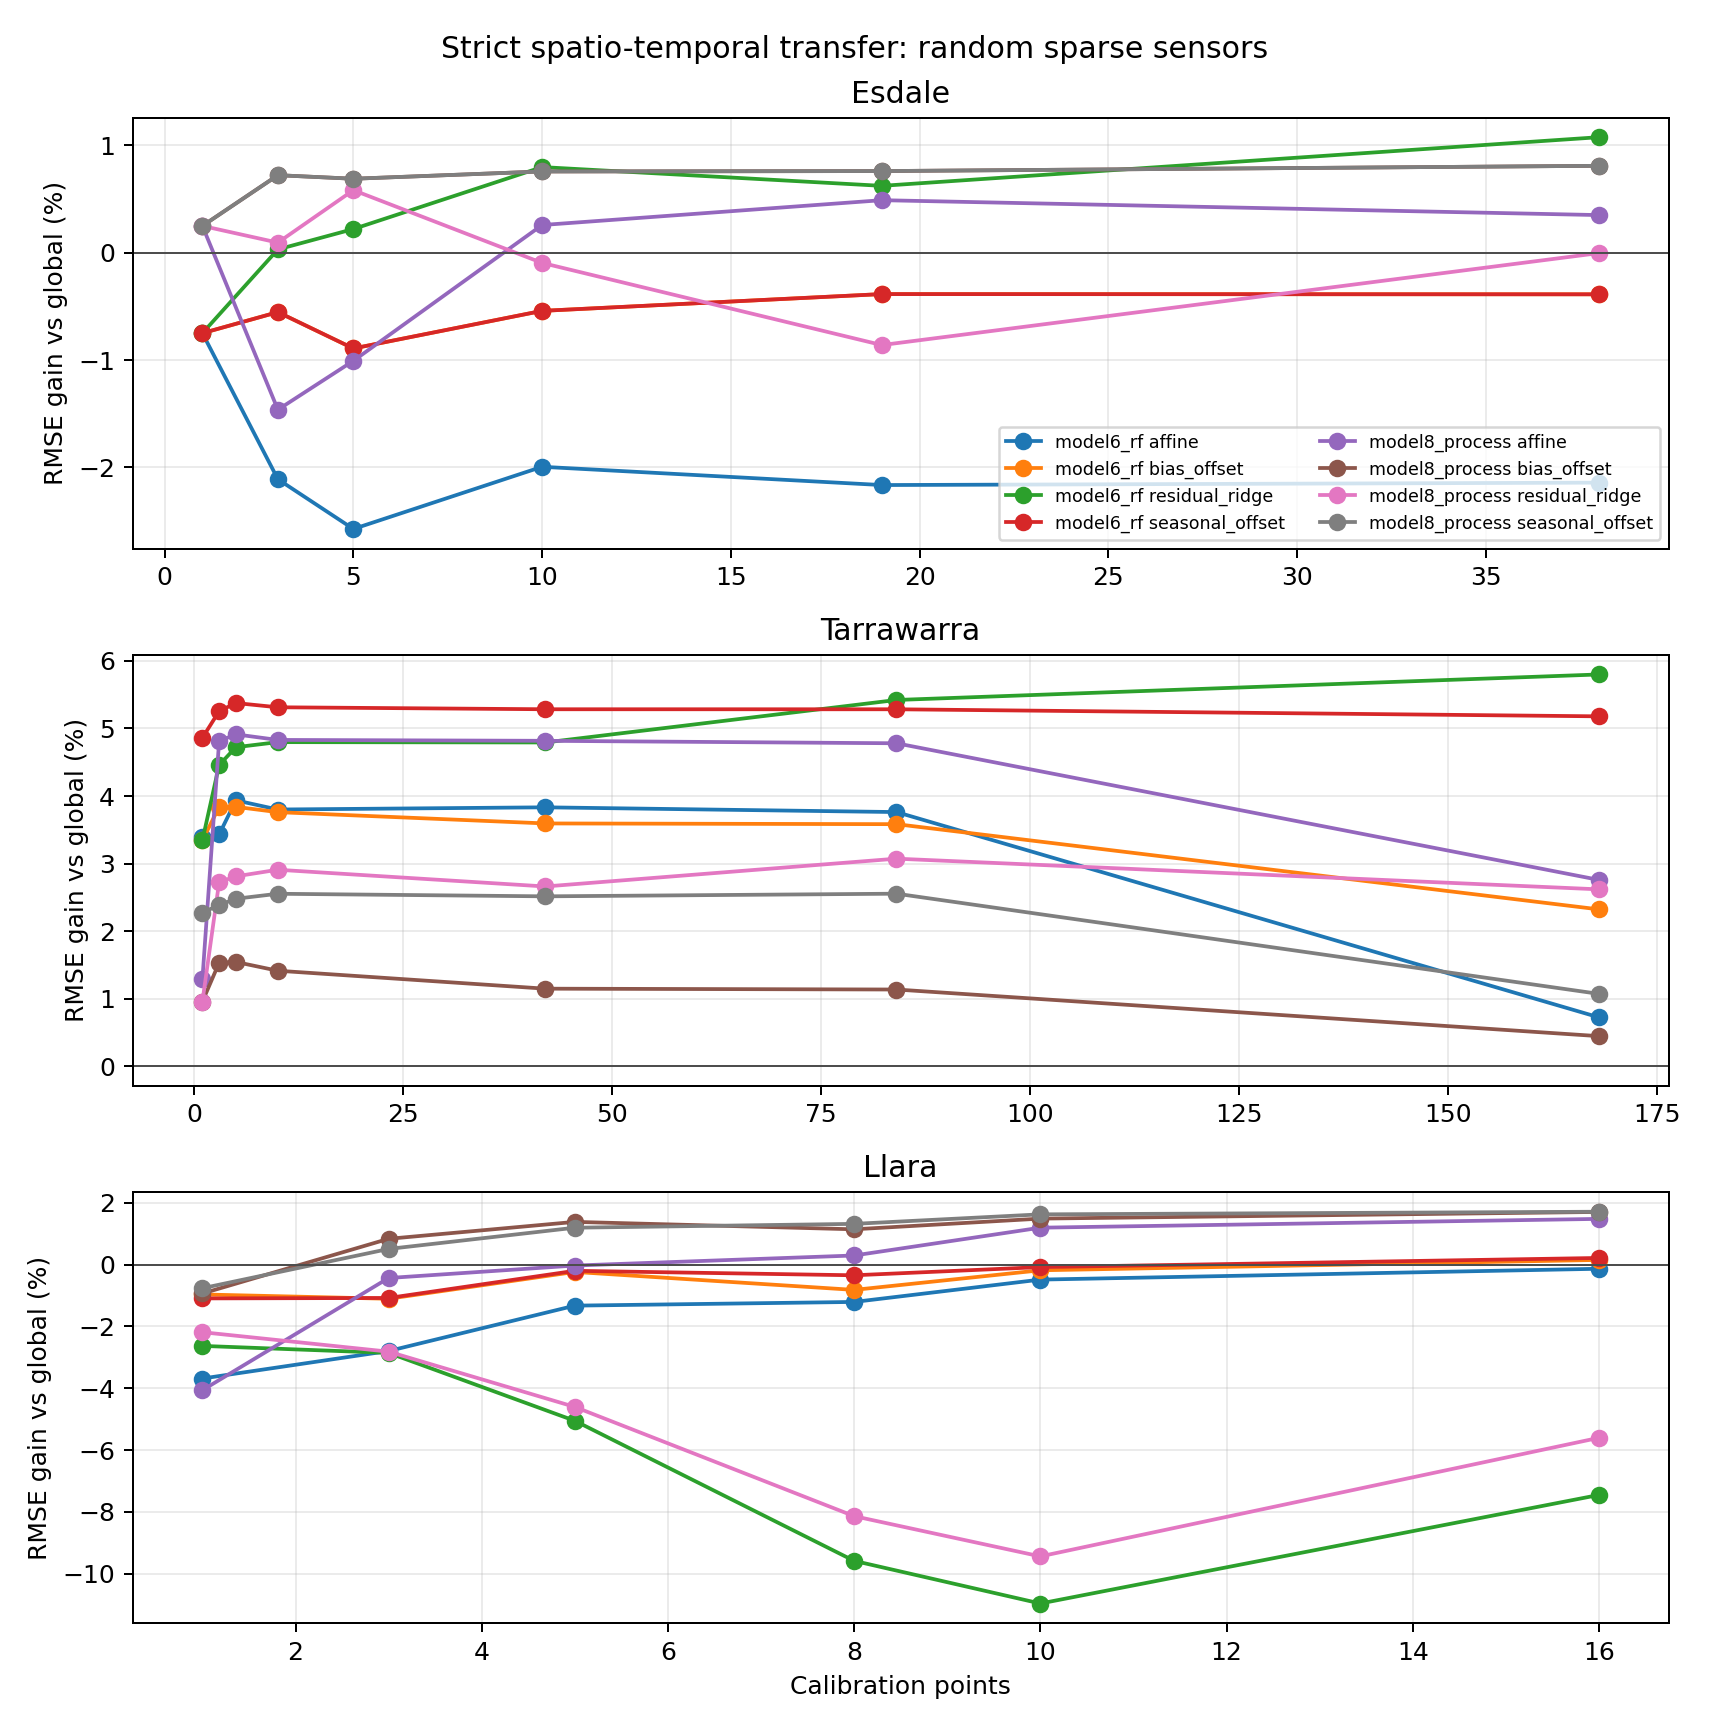
\includegraphics[width=\textwidth,height=0.82\textheight,keepaspectratio]{random_spatiotemporal_learning_curves_rmse_gain.png}
\caption{Appendix random-placement sparse local-calibration learning curves
under strict spatial+temporal blocking.  Positive values indicate lower RMSE
after calibration.}
\label{fig:app-random-rmse}
\end{figure}

\begin{figure}[htbp]
\centering
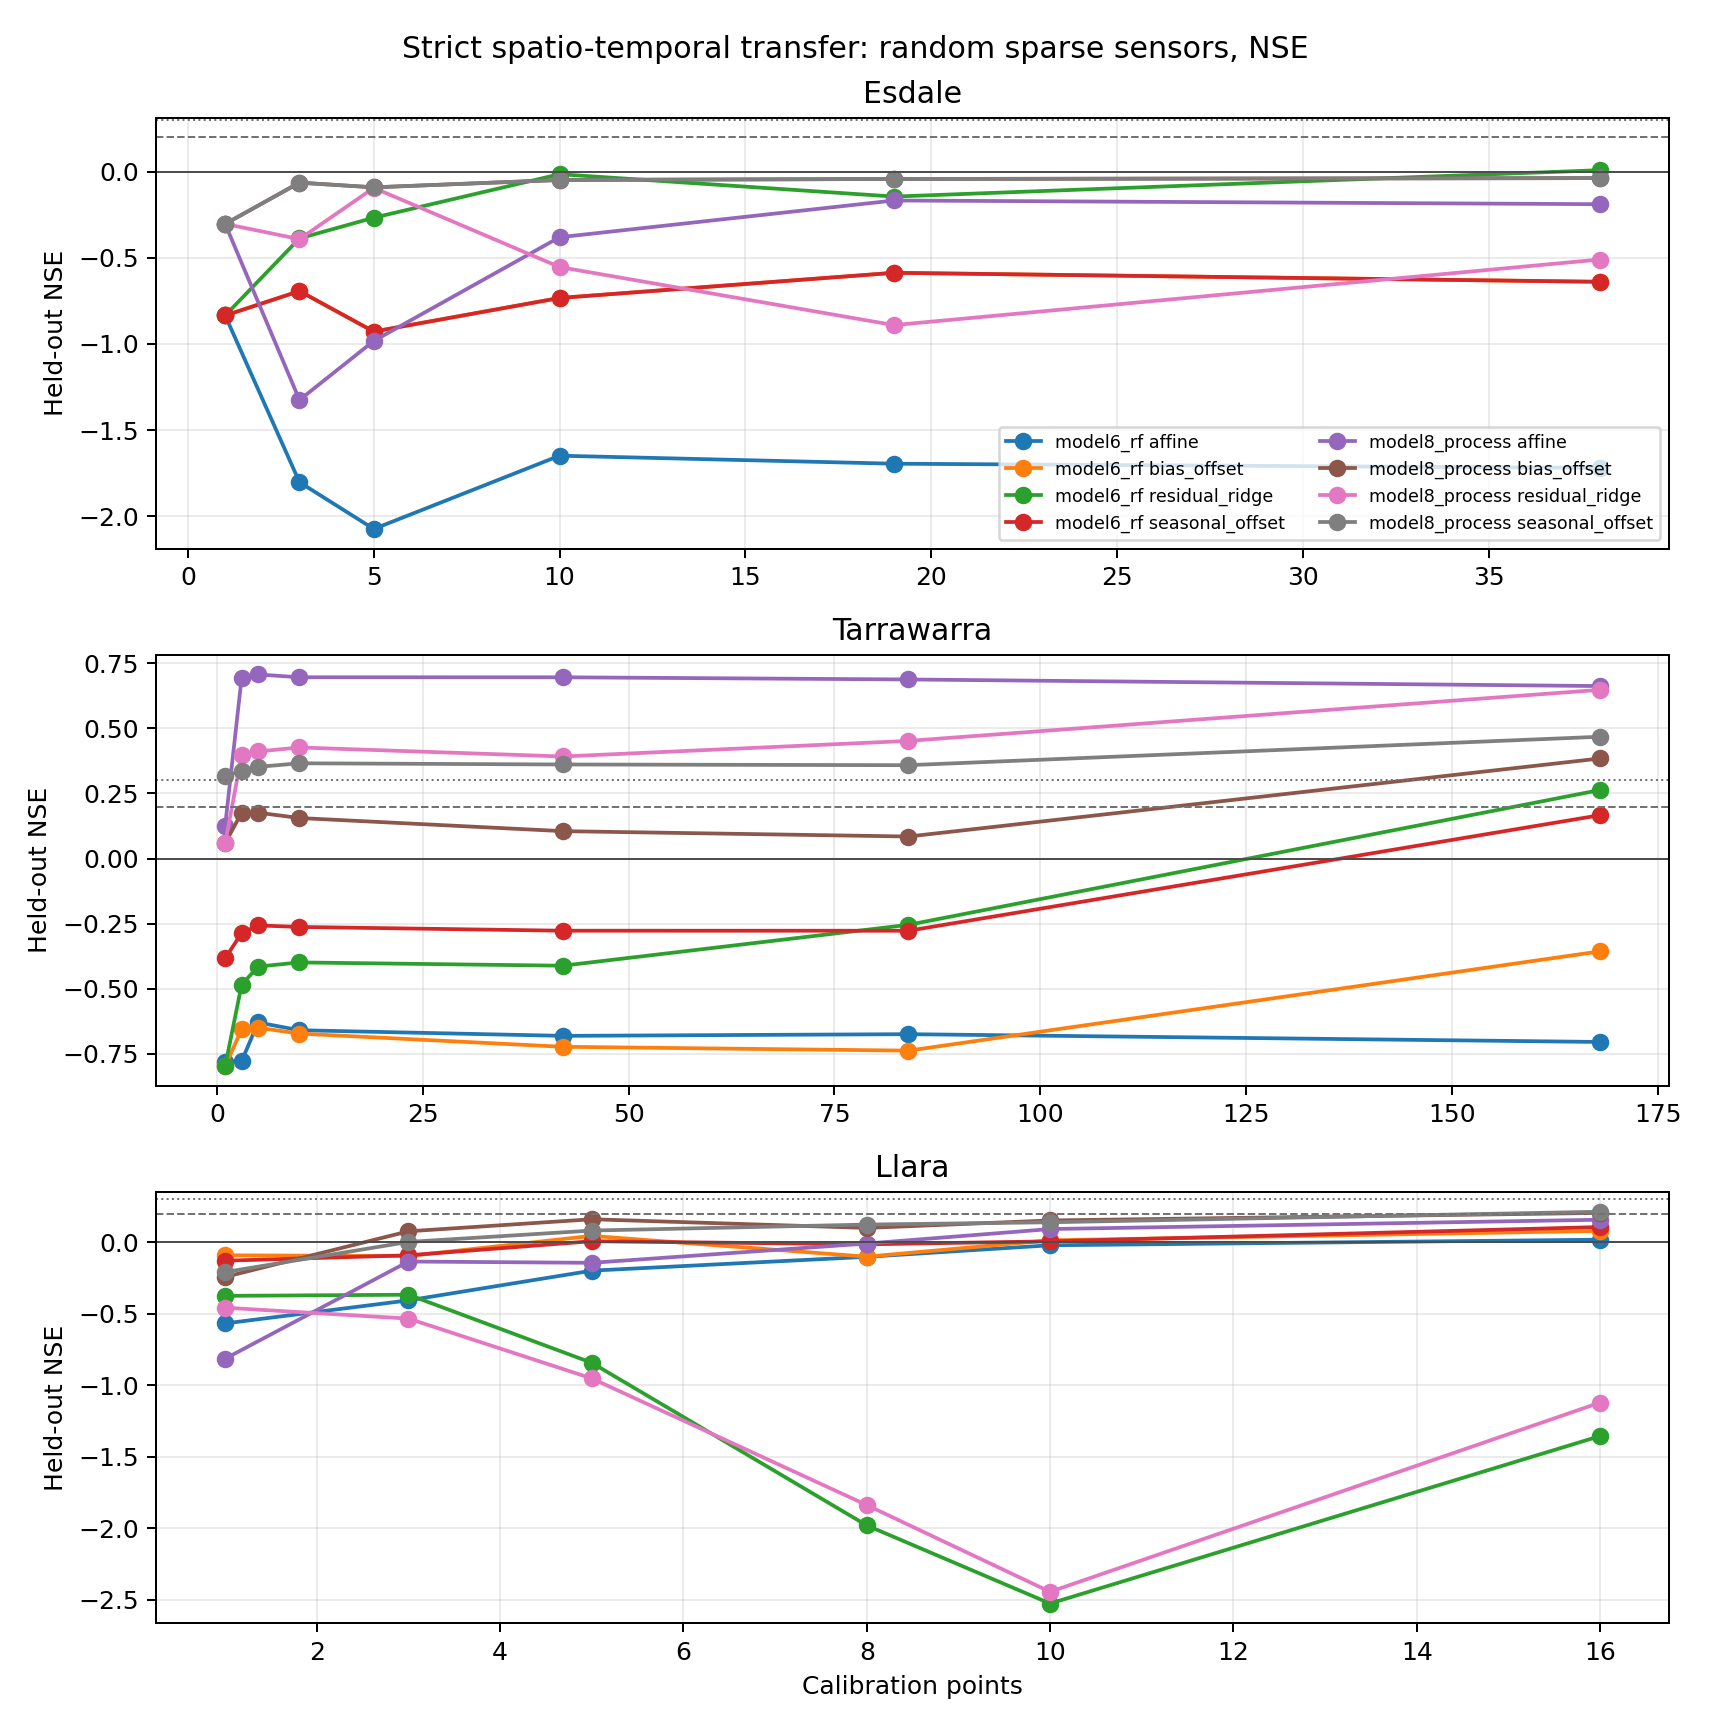
\includegraphics[width=\textwidth,height=0.82\textheight,keepaspectratio]{random_spatiotemporal_learning_curves_nse.png}
\caption{Appendix random-placement sparse local-calibration learning curves
expressed as held-out \nse{} under strict spatial+temporal blocking.}
\label{fig:app-random-nse}
\end{figure}

\begin{figure}[htbp]
\centering
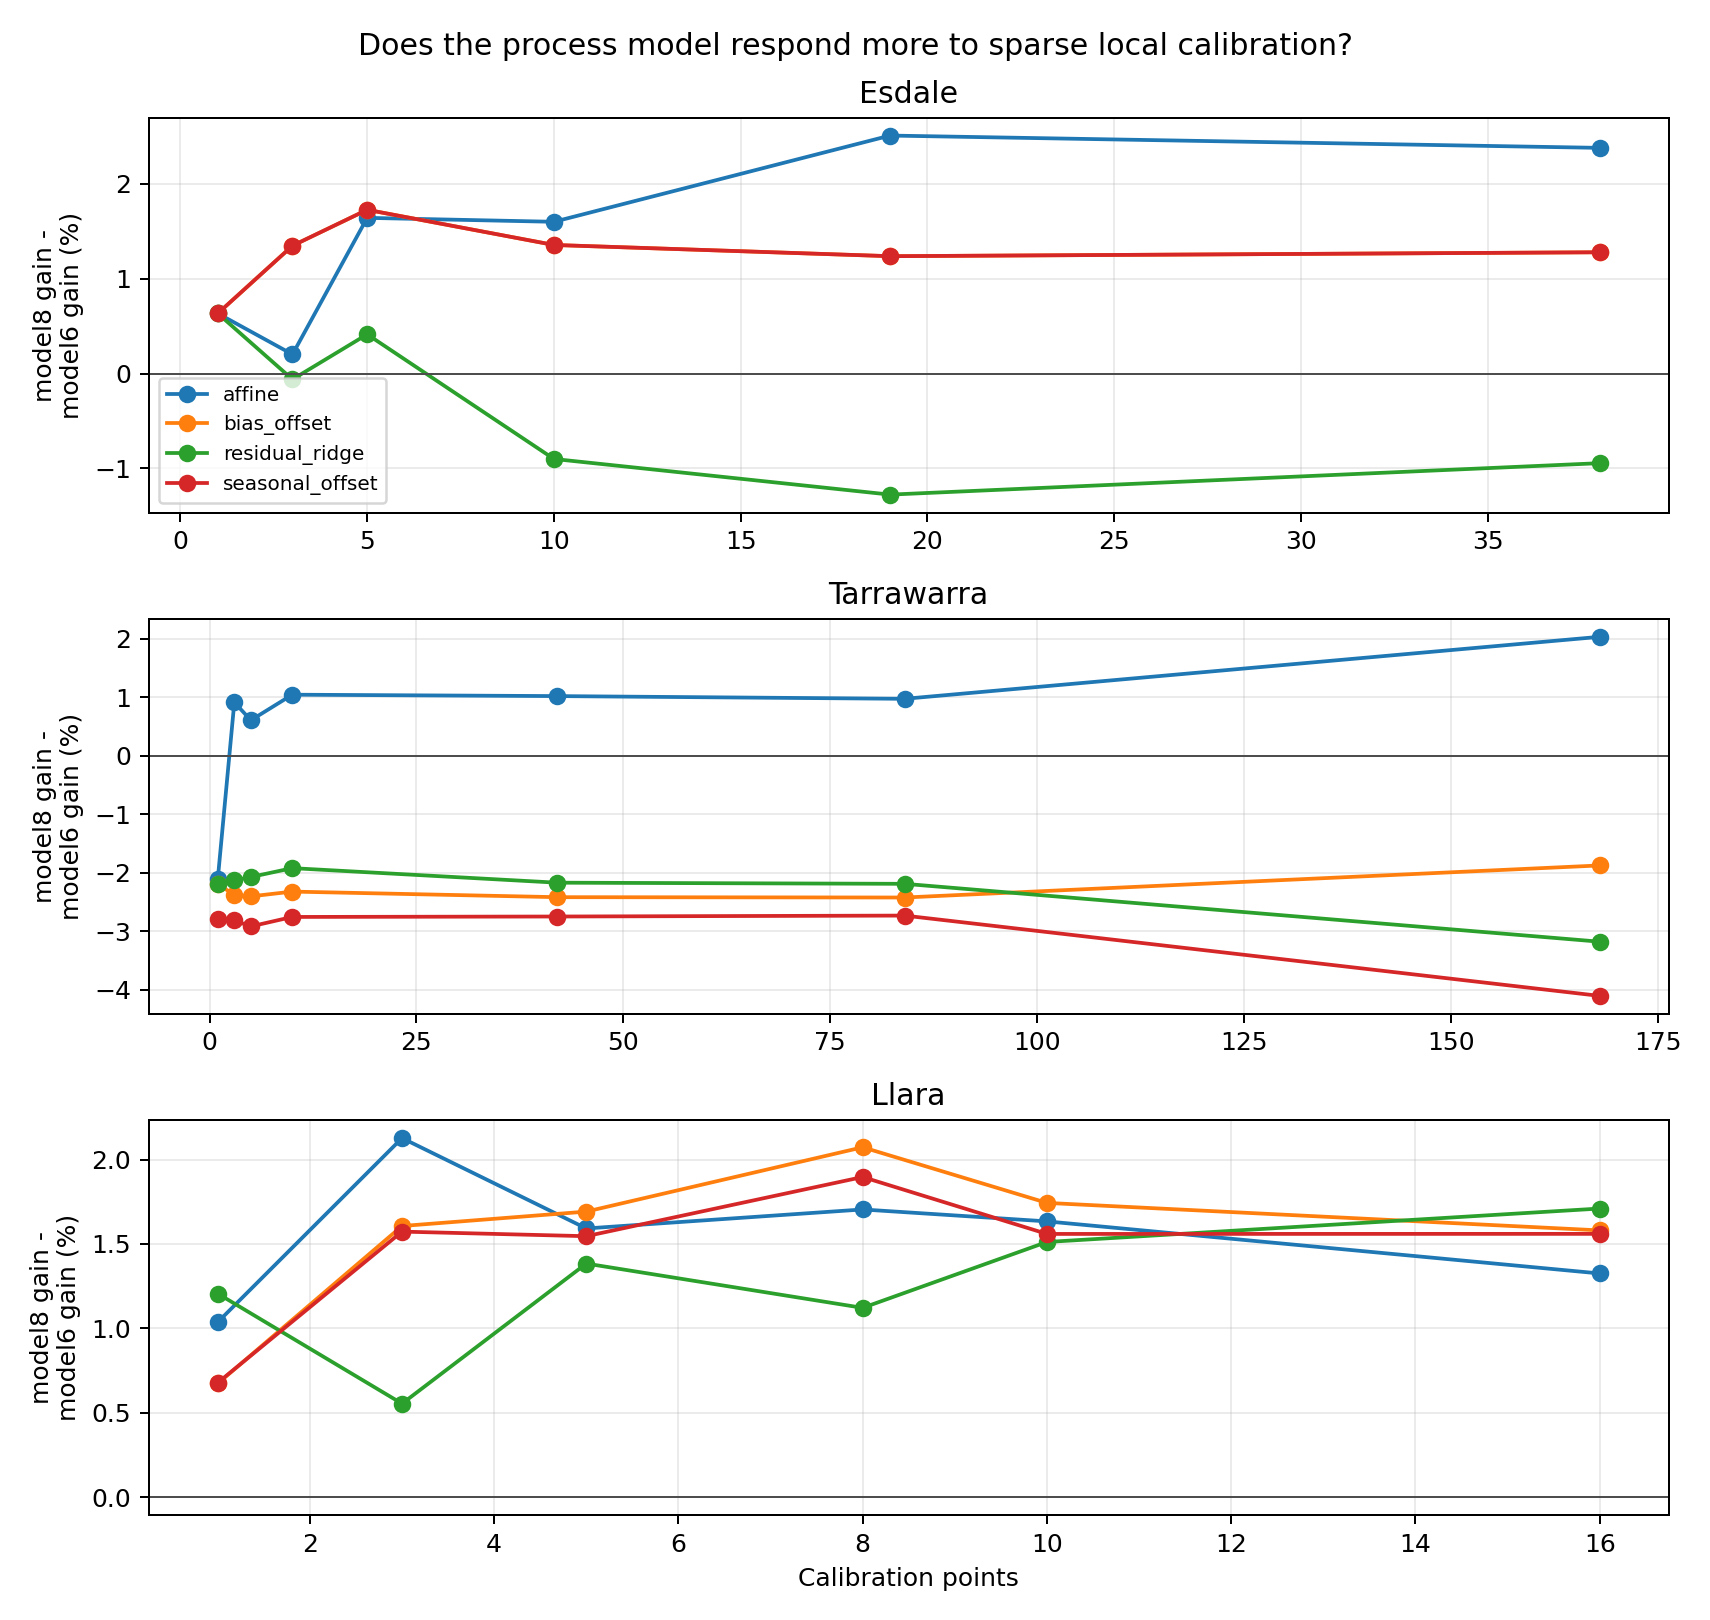
\includegraphics[width=0.9\textwidth,height=0.82\textheight,keepaspectratio]{process_vs_statistical_responsiveness_random.png}
\caption{Appendix process-vs-statistical local calibration responsiveness under
random placement.  Positive values indicate that \modelEight{} gained more RMSE
improvement than \modelSix{} from the same random sparse local information
budget.}
\label{fig:app-random-process}
\end{figure}

\bibliographystyle{plainnat}
\bibliography{../../../../DownscalingMoistureModel/paper/references,references_dense_validation}

\end{document}
